\documentclass[a4paper, 12pt]{article}
\usepackage[T1]{fontenc}
\usepackage{lmodern}
\usepackage{color}
\usepackage{amsfonts}
\usepackage{epstopdf}
\usepackage{matlab}
\usepackage{booktabs}
%\documentclass{book}
\usepackage{blindtext}
\usepackage{hyperref}
\usepackage[brazil]{babel}
\usepackage{amssymb}
\usepackage[utf8]{inputenc}
\usepackage{amsmath}
\usepackage{indentfirst}
\usepackage{graphicx}
\usepackage{listings}
\usepackage{tcolorbox}
\usepackage{upgreek}
\usepackage{multicol,lipsum}
\usepackage[a4paper,
top=3cm, left=3cm, bottom=3cm, right=3cm]{geometry}
\usepackage{setspace}
\usepackage{multirow}
\usepackage{float}
\usepackage[dvipsnames]{xcolor}
\usepackage[table]{xcolor}
%\usepackage{pdflscape}
\usepackage[DIV=15]{typearea}
\usepackage[nottoc]{tocbibind}
\usepackage[sort,numbers]{natbib}
%\usepackage{cite}
\usepackage{matlab}

\usepackage[utf8]{inputenc}
\usepackage[T1]{fontenc}
\usepackage{lmodern}
\usepackage{graphicx}
\usepackage{color}
\usepackage{hyperref}
\usepackage{amsmath}
\usepackage{amsfonts}
\usepackage{epstopdf}
\usepackage[table]{xcolor}
\usepackage{matlab}

\lstdefinestyle{python}{
  language=Python,
  basicstyle=\ttfamily,
  keywordstyle=\color{blue},
  stringstyle=\color{orange},
  commentstyle=\color{gray},
  numbers=left,
  numberstyle=\tiny\color{gray},
  stepnumber=1,
  numbersep=5pt,
  backgroundcolor=\color{white},
  showspaces=false,
  showstringspaces=false,
  showtabs=false,
  frame=single,
  rulecolor=\color{black},
  tabsize=4,
  captionpos=b,
  breaklines=true,
  breakatwhitespace=false,
  title=\lstname,
  escapeinside={\%*}{*)},
  morekeywords={self},
  emph={MyClass,__init__},
  emphstyle=\color{red}
}


\documentclass[letterpaper]{article}
% bib pack %%%%%%%%%%%%%%%%%%%%%%%%%%%%%%%%%%%%%%%%%%%%%%%%%%%%%%%%%%%%%%%%%%%%%
\usepackage[utf8]{inputenc}
\usepackage{geometry}
    \geometry{left=3cm,right=2cm,top=2cm,bottom=2cm}
%
\usepackage[spanish]{babel}
%
\usepackage[fixlanguage]{babelbib}
    \bibliographystyle{babunsrt}
%
\usepackage{url}

\begin{document}
%\maketitle

\begin{titlepage}
	\begin{center}
		

\vspace{10pt}
%\begin{figure}[H][!ht]
%\centering
%
\includegraphics{puc-rio-logo.png}

%\end{figure}
\begin{figure}[!ht]
\centering

\includegraphics{images/puc-rio-logo.png}
\end{figure}
\huge{Análise de Séries Temporais}
        \vspace{70pt}
        
		\textbf{ENG1469}
		\textbf{\large{\\ }}
		
		\vspace{30pt}
		\textbf{\small{\\Lista Prática 02}}
		\vspace{75pt}
		
	\end{center}
	
	\begin{flushleft}
		\begin{tabbing}
		Aluno(a)\qquad\qquad\=\>Paloma Fernanda Loureiro Sette - 1621595\\
			Professor(a)\>Cristiano Fernandes\\
	\end{tabbing}
		  
	\end{flushleft}
	\begin{center}
		%\vspace{\fill}
		\vspace{215pt}
		Rio de Janeiro, 20 de Outubro de 2024
	\end{center}
\end{titlepage}
%%%%%%%%%%%%%%%%%%%%%%%%%%%%%%%%%%%%%%%%%%%%%%%%%%%%%%%%%%%
\newpage
\tableofcontents
\thispagestyle{empty}

\newpage
\pagenumbering{arabic}

\newpage

%\newcommand{\listequationsname}{Lista de Equações}
%\newlistof{myequations}{equ}{\listequationsname}
%\newcommand{\myequations}[1]{%
%\addcontentsline{equ}{myequations}{\protect\numberline{\theequation}#1}\par}

%\listofmyequations
\newpage


\newpage

\listoffigures
\thispagestyle{empty}

\newpage
%%%%%%%%%%%%%%%%%%%%%%%%%%%%%%%%%%%%%%%%%%%%%%%%%%%%%%%%%
%%%%%%%%%%%%%%%%%%%%%%%%%%%%%%%%%%%%%%%%%%%%%%%%%%%

\newpage

\thispagestyle{empty}

\newpage

\section*{Introdução}
Este relatório refere-se à segundad lista prática da disciplina de Análise de Séries Temporais (ENG1469) de 2024.2.\\

Para este trabalho, utilizaremos a série temporal relacionada a vendas nominais no varejo de livros, jornais, revistas e papelaria. É possível encontrar esta série no \href{http://ipeadata.gov.br/Default.aspx}{Ipeadata}. (macroeconômico >> Periodicidade >> Mensal >> Consumo e Vendas >> Vendas nominais no varejo de livros, jornais, revistas e papelaria). Abaixo, apresentamos uma breve demonstração de como chegar até a base de dados utilizada. Esta demonstração se deve ao fato de que, por algum motivo, o site do Ipeadata não nos gera o link exato até a base (ou seja, qualquer endereço que copiamos é sempre http://ipeadata.gov.br/Default.aspx).\\



\begin{figure}[H]
\centering
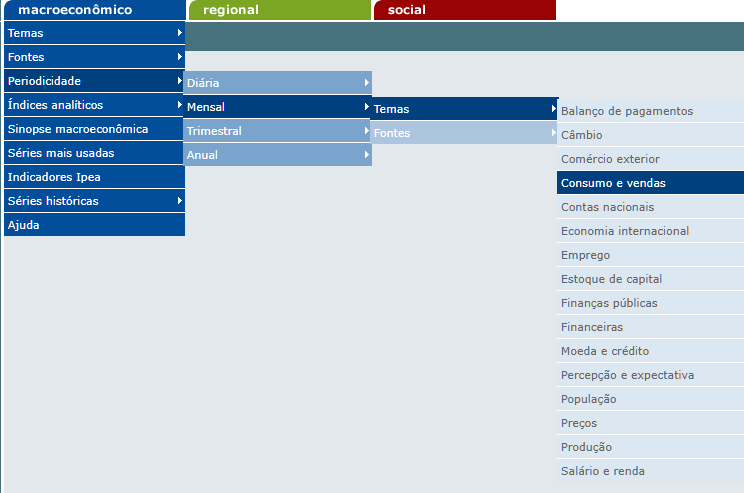
\includegraphics[scale = 0.65]{images/caminho_ipeadata.png}
\label{filtro1}
\caption{Ipeadata - caminho até a base de dados}
\end{figure}

\begin{figure}[H]
\centering
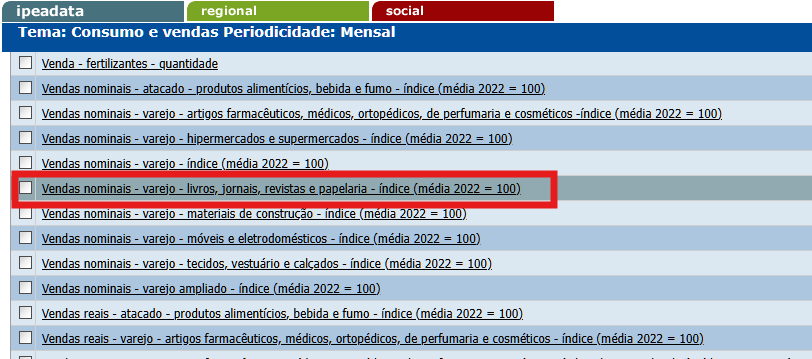
\includegraphics[scale = 0.65]{images/ipeadata_caminho2.png}
\label{filtro1}
\caption{Ipeadata - base de dados utilizada}
\end{figure}

Para vendas nominais, considera-se a receita bruta de revenda, total e por Unidade da Federação, definida no âmbito da empresa como a receita bruta mensal proveniente da revenda de mercadorias, não deduzidos os impostos incidentes e nem as vendas canceladas, abatimentos e impostos incondicionais. Para varejo considera-se as atividades de revenda, venda sem transformação significativa, de bens de consumo novos e usados, preponderantemente para o consumidor final. O comércio varejista é organizado para vender mercadorias em pequenas quantidades ao consumidor final, representando, portanto, o último elo da cadeia de distribuição. A classificação das atividades do comércio varejista baseia-se na gama de produtos vendidos, sem distinção da forma de comercialização em loja ou fora de loja. Para livros, jornais, revistas e papelaria considera-se o comércio varejista de livros, inclusive didáticos, o comércio varejista de revistas, jornais, revistas e outros impressos, o comércio varejista de artigos de escritório, as bancas de jornais e revistas, o comércio varejista de artigos de papelaria, tais como cadernos, borrachas, lápis, canetas, cartolinas e similares. Não fazendo parte desta classificação o comercio varejista de livros usados, o comércio varejista de selos, o comércio varejista de suprimentos de informática. A base foi fixada como a média das observações no ano de 2022. Nota: A Pesquisa Mensal de Comércio foi iniciada em janeiro de 1995, com o intuito de produzir indicadores que possam acompanhar o desempenho conjuntural do comércio varejista no país, investigando a receita bruta de revenda nas empresas formalmente constituídas de 20 ou mais pessoas ocupadas.\\

\newpage
\subsection{Carregando os dados}
A princípio, é necessário carregar os dados e fazer os devidos tratamentos:

\begin{lstlisting}[style=python]
import pandas as pd

file_path = 'dados.xls' 

data = pd.read_excel(file_path)

data['Data'] = data['Data'].astype(str)

data['Data'] = pd.to_datetime(data['Data'], format='%Y.%m')

data.set_index('Data', inplace=True)

# Dividindo a serie em treino e teste
train = data.iloc[:-12]  # Todas as observacoes exceto as 12 ultimas
test = data.iloc[-12:]   # As ultimas 12 observacoes

\end{lstlisting} \\

No código acima, carregamos os dados do documento XLS original, que contém as colunas Data e Vendas, e dividimos a série em dados de treino e teste. 

\begin{figure}[H]
\centering
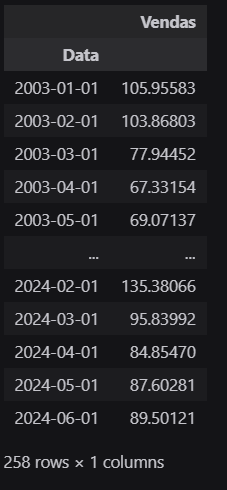
\includegraphics[scale = 0.80]{images/0.1.png}
\label{filtro1}
\caption{Dataframe base - ST}
\end{figure}

\newpage
\subsection{Especificações}

Para melhor especificar os dados da série, implementamos a tabela abaixo, cujos dados referem-se a:

\begin{itemize}
    \item Data do início e do fim;
    \item Data de início e fim do período de treinamento;
    \item Data de início e fim do período de teste;
    \item Unidade de medida;
    \item Fonte de dados.
\end{itemize}

\begin{table}[htbp]
\centering
\begin{tabular}{|l|l|}
\hline
\textbf{Descrição}                                        & \textbf{Detalhes}                    \\ \hline
Data de início e fim da série                             & 2003-01-01 - 2024-06-01              \\ \hline
Data de início e fim do período de treinamento            & 2003-01-01 - 2023-06-01              \\ \hline
Data de início e fim do período de teste                  & 2023-06-01 - 2024-06-01              \\ \hline
Unidade de medida                                          & Índice (média 2022 = 100)            \\ \hline
Fonte de dados                                             & IPEADATA                             \\ \hline
\end{tabular}
\caption{Especificações da Série Temporal}
\end{table}




%%%%%%%%%%%%%%%%%%%%%%%%%%%%%%%%%%%%%%%%%%%%%%%%%
\newpage
\section{- Questão 01}


\subsection{Questão 1: Parte (i)}
\textbf{Obtenha o gráfico da série no tempo, da sua 1a diferença e da sua 2a diferença. A partir
desses gráficos determine, informalmente, o valor do parâmetro “d” (ordem de integração não
sazonal), justificando a sua escolha. Escreva a expressão da série diferenciada utilizando o
operador de atraso L, denominando essa série de zt
, sendo yt
 a série original.} \\

\subsubsection{Análise Gráfica da Série Temporal e Diferenças}

A série temporal original, composta por dados de vendas nominais, apresenta uma tendência clara e sazonalidade marcante, como evidenciado no gráfico. Ao aplicar a primeira e segunda diferenciação, observamos a eliminação progressiva das tendências, o que é esperado ao tentarmos tornar a série estacionária.\\

A visualização dos gráficos, entretanto, apresenta alguns desafios. Em comparação com plataformas como o IPEADATA, o gráfico gerado pelo Python exibe "nós" e sobreposições mais densas. Isso se deve a uma combinação de fatores:\\

\textbf{Resolução e Tamanho do Gráfico}: Os gráficos gerados em Python, por padrão, podem ter resoluções mais baixas, o que faz com que as linhas e os dados se apresentem mais "apertados". Embora o código tenha sido ajustado para melhorar a largura das linhas e o espaçamento dos eixos, ainda existem limitações que afetam a suavidade visual.\\

\textbf{Densidade dos Dados}: A série contém um grande número de observações (anos de vendas mensais), e, ao plotar todos esses pontos de dados, é natural que os gráficos resultem em sobreposições. Em gráficos interativos ou gerados em maior resolução, esses pontos podem ser melhor explorados e analisados.\\

\textbf{Rotação de Rótulos e Ajustes de Layout}: Mesmo com a rotação de rótulos no eixo X, a densidade de dados ainda pode causar certa confusão visual em gráficos estáticos. Ferramentas interativas permitem que o observador foque em detalhes específicos, o que não é possível em gráficos estáticos como o gerado aqui.\\

Apesar dessas limitações, os gráficos permitem uma análise adequada da estacionaridade da série ao observar que a primeira diferenciação não elimina completamente a sazonalidade, mas torna a série mais estável. A segunda diferenciação parece eliminar mais oscilações, o que nos sugere que o valor de $d$ poderia ser 1 ou 2, dependendo da modelagem.\\

\begin{figure}[H]

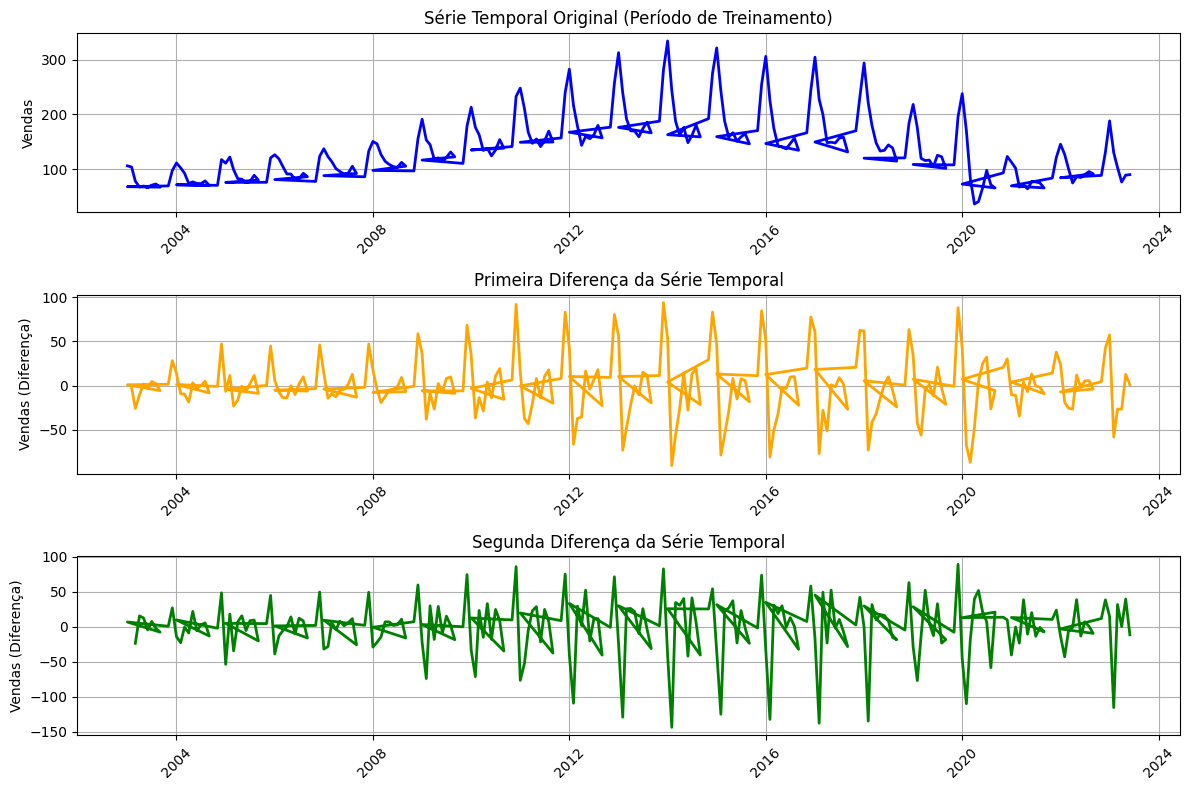
\includegraphics[scale = 0.5]{images/graficos_1_i.png}
\label{filtro1}
\caption{Gráficos plotados da série e primeira e segunda diferenças}
\end{figure}

\begin{figure}[H]
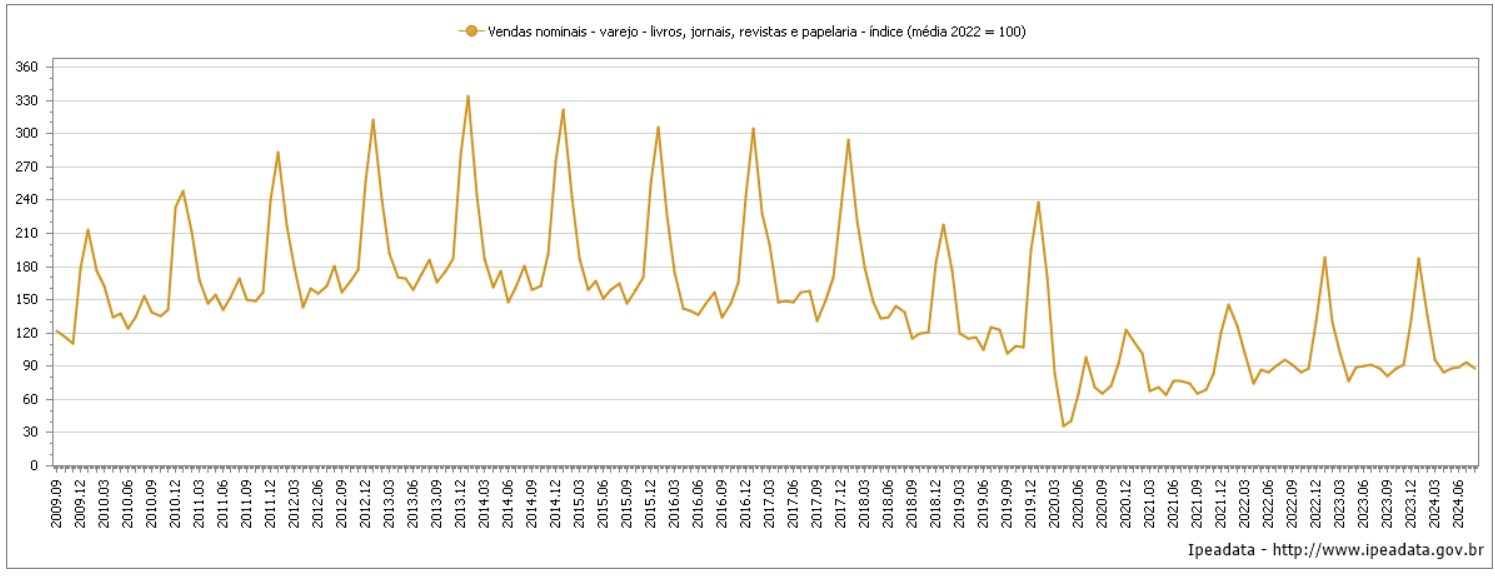
\includegraphics[scale = 0.4]{images/grafico_ipeadata.jpg}
\label{filtro1}
\caption{Gráfico do site Ipeadata}
\end{figure}

A partir da análise gráfica da série temporal original, da primeira e da segunda diferenciação, podemos determinar informalmente o valor do parâmetro \(d\) (ordem de integração não sazonal) da seguinte maneira:

\begin{itemize}
    \item A série temporal original apresenta uma clara tendência, o que indica que a série não é estacionária. Portanto, uma diferenciação é necessária para remover essa tendência.
    \item Após a primeira diferenciação, observamos que a série apresenta comportamento mais estacionário, removendo a tendência, mas mantendo um padrão sazonal. Isso indica que uma única diferenciação é suficiente para remover a não-estacionaridade associada à tendência. A sazonalidade será tratada separadamente com o componente sazonal.
    \item Após a segunda diferenciação, a série apresenta menor variabilidade, mas não é necessário aplicar mais uma diferenciação para remover a sazonalidade.
\end{itemize}

Com base nessa análise, determinamos que o valor de \(d\) é 1, pois a primeira diferenciação já remove a tendência e torna a série estacionária em termos de tendência.

\subsubsection{Expressão da Série Diferenciada}

A expressão da série temporal diferenciada pode ser representada utilizando o operador de atraso \(L\). O operador \(L\) desloca a série temporal em um período, ou seja, \(L^k y_t = y_{t-k}\), onde \(y_t\) é a série original.\\

A primeira diferença de \(y_t\) pode ser representada como:

\[
z_t = y_t - L y_t = (1 - L) y_t
\]

Portanto, a série \(z_t\), que é a primeira diferenciação da série \(y_t\), pode ser expressa como:

\[
z_t = (1 - L) y_t
\]

\noindent Como a série já se torna estacionária após a primeira diferenciação, não há necessidade de aplicar uma segunda diferenciação.

\subsubsection{Justificativa do Valor de \(d = 1\)}

Conforme a análise gráfica e os conceitos discutidos, o valor \(d = 1\) é justificado pela remoção da tendência após a primeira diferenciação. A sazonalidade será tratada pelo componente sazonal do modelo SARIMA (\(D\)), evitando a necessidade de mais uma diferenciação. A ordem de integração não sazonal \(d = 1\) é suficiente para modelar a série temporal, conforme observado.\\\\


\subsection{Questão 1: Parte (ii)}
\textbf{Realizar o teste KPSS para escolher o valor da ordem de diferenciação não sazonal da
série, “d”. Especificar Ho, Ha e o resultado do teste. Comparar esse valor de “d” com aquele
que vc sugerimos em i). Para esse valor de “d”, obter a série diferenciada, seguida da FAC e
FACP.}

\subsubsection{Teste KPSS para verificar a estacionaridade da série e determinar $d$}

O teste KPSS tem como hipótese nula $H_o$ que a série é estacionária, e a hipótese alternativa $H_a$ é que a série não é estacionária.\\

Executamos o seguinte script em Python para realizar o teste KPSS e obter o valor $d$: 

\begin{lstlisting}[style=python]
""" Parte (ii) """

# Realizar o teste KPSS na serie original (nao diferenciada)
kpss_test = kpss(train['Vendas'], regression='c', nlags='auto')

# Exibir os resultados do teste KPSS
print(f'KPSS Test Statistic: {kpss_test[0]}')
print(f'p-value: {kpss_test[1]}')
print(f'Critical Values: {kpss_test[3]}')

# Interpretacao
if kpss_test[1] < 0.05:
    print("A serie NAO eh estacionaria (Rejeita H0)")
else:
    print("A serie e estacionaria (Aceita H0)")
    \end{lstlisting} \\

Onde obtivemos os seguintes resultados:

\begin{figure}[H]
\centering
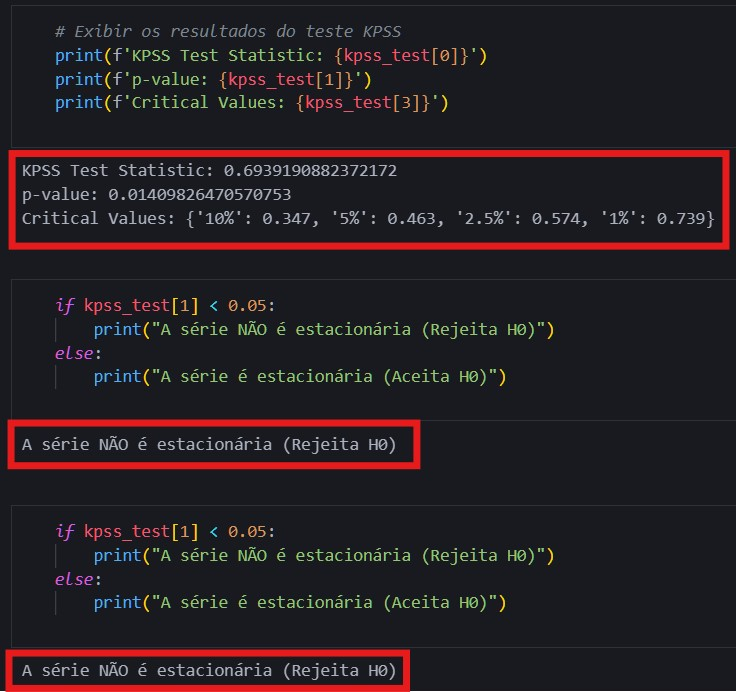
\includegraphics[scale = 0.55]{images/results-kpss.jpg}
\label{filtro1}
\caption{Resultado - KPSS}
\end{figure}

\subsubsection{AC (Função de Autocorrelação) e FACP (Função de Autocorrelação Parcial)}

Após determinar $d$, o próximo passo é obter as funções de autocorrelação (FAC) e autocorrelação parcial (FACP) para entender os padrões sazonais da série.\\

O código para gerar os gráficos da FAC e FACP foi implementado da seguinte forma:

\begin{lstlisting}[style=python]
# Serie diferenciada com base no valor de 'd'
differenced_series = train['Vendas'].diff().dropna()

# Plotar a FAC e a FACP da serie diferenciada
plt.figure(figsize=(12, 6))

# FAC
plt.subplot(1, 2, 1)
plot_acf(differenced_series, lags=36, ax=plt.gca(),
         title='FAC - Serie Diferenciada')

# FACP
plt.subplot(1, 2, 2)
plot_pacf(differenced_series, lags=36, ax=plt.gca(),
          title='FACP - Serie Diferenciada')

plt.tight_layout()
plt.show()
    \end{lstlisting} \\

Onde obtivemos os seguintes resultados:

\begin{figure}[H]
\centering
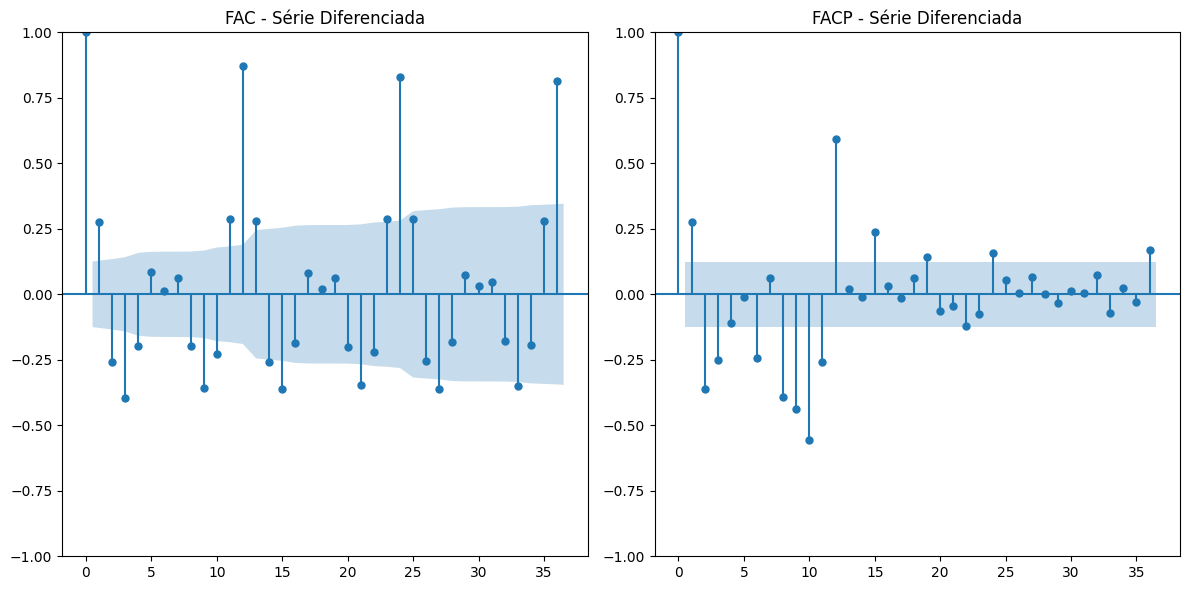
\includegraphics[scale = 0.5]{images/FAC_FACP_1_ii.png}
\label{filtro1}
\caption{Gráficos da FAC e FACP}
\end{figure}

\subsubsection{(a) Existe dependência sazonal nessa série?}

Sim, existe dependência sazonal na série, conforme evidenciado pelos picos significativos observados na Função de Autocorrelação (FAC) nas defasagens sazonais, ou seja, múltiplos de 12 (\(k = 12, 24, 36\)). Esses picos indicam que existe uma correlação significativa em intervalos temporais sazonais, o que caracteriza uma forte dependência sazonal na série temporal.


\subsubsection{(b) É possível sugerir um modelo ARIMA(p,d,q), de partida, para a série $y_t$?}

Sim, é possível sugerir um modelo ARIMA \((p,d,q)\) de partida para a série \(y_t\). Com base nos gráficos da Função de Autocorrelação Parcial (FACP), observam-se picos significativos nos primeiros lags, sugerindo um possível valor para \(p\). A ausência de padrões de decaimento abrupto na FAC indica que o valor de \(q\) não precisa ser elevado. Assim, um modelo ARIMA \((1,1,1)\) pode ser sugerido como um ponto de partida, sendo que \(d = 1\) foi determinado pelo teste KPSS, que revelou a necessidade de uma diferenciação para tornar a série estacionária.


\subsubsection{(c) O padrão de decaimento da FAC nos lags sazonais sugere a necessidade  de diferenciação sazonal “D” para a série, além de “d”?}

Sim, o padrão de decaimento da FAC nas lags sazonais \(k = 12, 24, 36\) sugere a necessidade de uma diferenciação sazonal, ou seja, \(D > 0\). Esses picos em múltiplos de 12 indicam que a série contém uma componente sazonal significativa, mesmo após a primeira diferenciação não sazonal (\(d = 1\)). Portanto, recomenda-se aplicar uma diferenciação sazonal de ordem \(D = 1\) para capturar essa sazonalidade presente na série.\\\\



\subsection{Questão 1: Parte (iii)}
\textbf{Obtenha o melhor “modelo não-sazonal” para a sua série original yt. Para isso utilize, no seu
software, o procedimento automático para selecionar o melhor modelo ARIMA(p,d,q) via AICc,
sem incluir lags sazonais, e fixando o “d” e “D” nos valores selecionados anteriormente (vc
deve informar na função que faz a busca automática que a busca não inclui lags sazonais; a
função auto.arima do R tem essa possibilidade).}\\

Nesta parte, vamos começar usando a função "auto\_arima" da biblioteca \textit{pdmarima}, que suporta a seleção de modelos ARIMA com base no AICc. Precisamos nos certificar também de ajustar para que não seja considerada a sazonalidade.\\

Para encontrar o melhor modelo não-sazonal para a série \(y_t\), utilizamos o procedimento de busca automática pelo critério AICc, conforme solicitado. Para isso, utilizamos o código Python baseado na função \texttt{auto\_arima} da biblioteca \texttt{pmdarima}, que permite ajustar modelos ARIMA automaticamente com base em diversos critérios de informação, como o AICc.\\

O código utilizado foi o seguinte:

\begin{lstlisting}[style=python]
import pmdarima as pm

""" Parte iii"""
# Ajustar o modelo ARIMA nao-sazonal com base no AICc
model = pm.auto_arima(train['Vendas'],
                      start_p=0, max_p=5,
                      start_q=0, max_q=5,
                      d=1,   #d foi escolhido antes como 1
                      seasonal=False,  #Ignorar sazonalidade
                      information_criterion='aicc',  #Criterio AICc
                      trace=True,
                      stepwise=True)

# Exibindo o resumo do modelo
print(model.summary())

# Valor de AICc
aicc_value = model.aicc()
print(f"Valor do AICc: {aicc_value}")
    \end{lstlisting} \\

Esse código realiza o ajuste do modelo ARIMA não-sazonal, com \(d = 1\) definido previamente e a busca pelos valores de \(p\) e \(q\) variando de 0 a 5. O critério de seleção foi o AICc, que penaliza modelos mais complexos, sendo ideal para a escolha de modelos de séries temporais. O código também ignorou a sazonalidade (\texttt{seasonal=False}), como especificado na questão. O valor de \(d = 1\) foi escolhido com base na análise anterior (parte i), onde determinamos que a série precisava de uma diferenciação não-sazonal.



\begin{figure}[H]
\centering
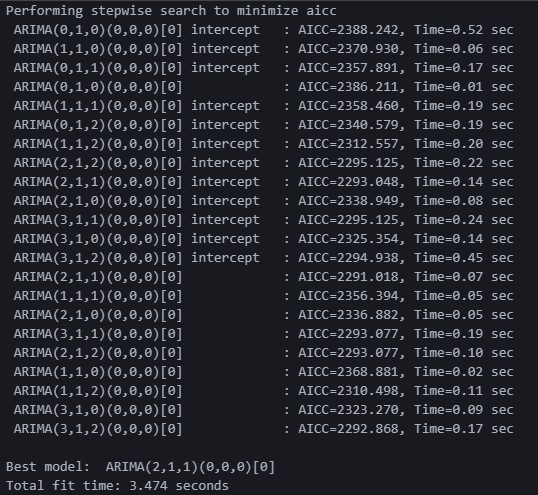
\includegraphics[scale = 0.85]{images/performing_sarima_1pt3.jpg}
\label{filtro1}
\caption{Performing stepwise search to minimize aicc}
\end{figure}




\subsubsection{(a) Melhor modelo e valor do AICc}

Após rodar o código, o modelo selecionado foi um \textbf{ARIMA(2,1,1)}, conforme a tabela de resultados gerada:

\begin{figure}[H]
\centering
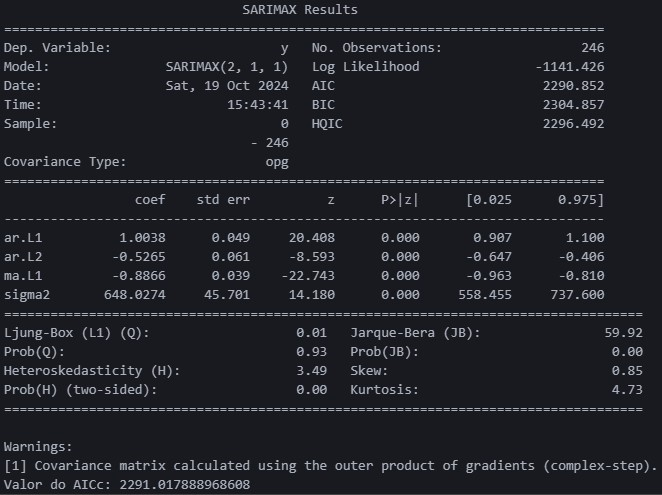
\includegraphics[scale = 0.85]{images/sarimax_results_pt3_q1.jpg}
\label{filtro1}
    \caption{Tabela de resultados - SARIMA}
\end{figure}

\[
\text{SARIMA}(2,1,1)(0,0,0)_{12}
\]

A equação SARIMA correspondente ao modelo ajustado é a seguinte:

\[
(1 - 1.0038 L + 0.5265 L^2)(1 - L) y_t = (1 + 0.8866 L) \epsilon_t
\]

Neste caso:
\begin{itemize}
    \item \(p = 2\): O modelo ARIMA selecionou dois termos autorregressivos.
    \item \(d = 1\): Foi aplicada uma única diferenciação para tornar a série estacionária.
    \item \(q = 1\): Um termo de média móvel foi selecionado.
    \item \(P = 0, D = 0, Q = 0\): Não houve inclusão de componentes sazonais.
\end{itemize}


O valor do \textbf{AICc} foi \textbf{2291.01789}, indicando o melhor modelo ajustado segundo esse critério.

\subsubsection{(b) Análise da FAC e FACP dos resíduos}

Após o ajuste do modelo ARIMA, obtivemos os resíduos do modelo para analisar se restaram padrões de dependência não explicados. O código utilizado para calcular a FAC e FACP dos resíduos foi:

\begin{lstlisting}[style=python]
# Obter os resíduos do modelo ajustado
residuals = model.resid()

# Plotar a FAC e FACP dos resíduos
plt.figure(figsize=(12, 6))

# FAC dos resíduos
plt.subplot(1, 2, 1)
plot_acf(residuals, lags=36, ax=plt.gca(), title='FAC dos Resíduos')

# FACP dos resíduos
plt.subplot(1, 2, 2)
plot_pacf(residuals, lags=36, ax=plt.gca(), title='FACP dos Resíduos')

plt.tight_layout()
plt.show()
    \end{lstlisting} \\


Os gráficos gerados (FAC e FACP) nos ajudam a observar se ainda existem padrões remanescentes de correlação nos resíduos, tanto em lags de curto prazo quanto em lags sazonais.\\\\

\textbf{Resultados da FAC e FACP dos Resíduos:}\\


\begin{figure}[H]
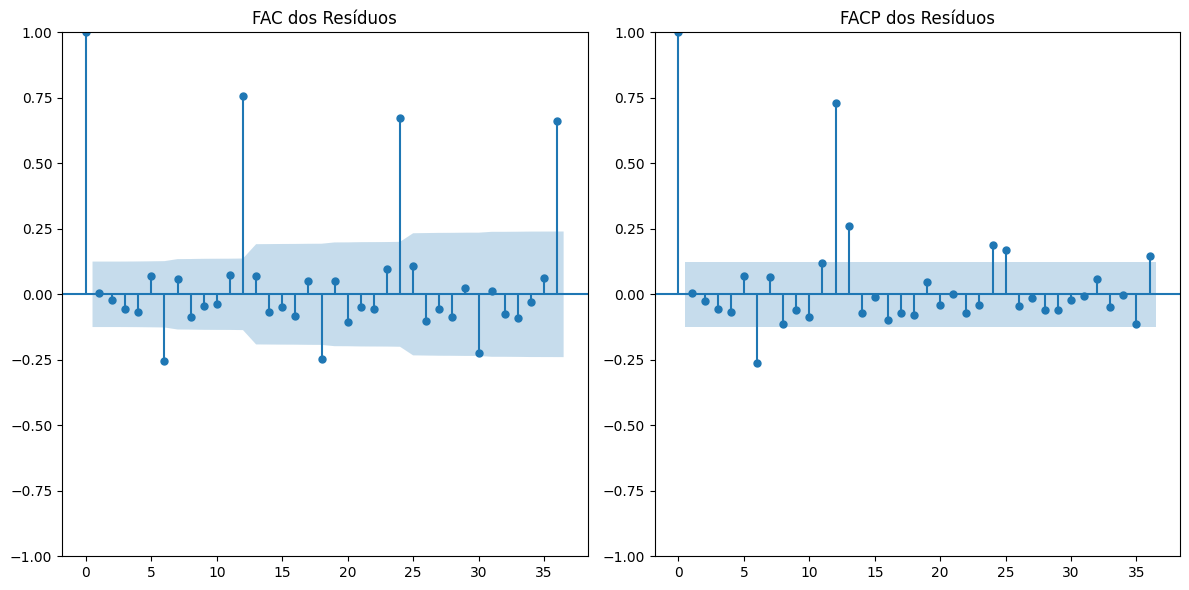
\includegraphics[scale = 0.5]{images/fac_facp_residuos.png}
\label{filtro1}
    \caption{Gráficos da FAC e da FACP dos resíduos}
\end{figure}

A seguir, analisamos os valores da Função de Autocorrelação (FAC) e da Função de Autocorrelação Parcial (FACP) dos resíduos do modelo ajustado, com foco nos lags de curto prazo \(k = 1, 2, 3, 4\) e no lag sazonal \(k = 12\), conforme solicitado.

\subsubsection*{FAC dos Resíduos}
\begin{itemize}
    \item Para os lags de curto prazo \(k = 1, 2, 3, 4\), a FAC dos resíduos mostra que os valores estão todos dentro dos limites de confiança. Isso indica que o modelo ARIMA(2,1,1) foi eficaz em capturar as correlações de curto prazo da série, não deixando dependências remanescentes nesses lags.
    \item No entanto, para o lag sazonal \(k = 12\), observamos um pico significativo fora dos limites de confiança, sugerindo que o modelo não conseguiu capturar adequadamente a dependência sazonal presente na série. Além disso, um pico similar ocorre no lag \(k = 24\), o que pode reforçar a ideia de uma dependência sazonal residual.
\end{itemize}

\subsubsection*{FACP dos Resíduos}
\begin{itemize}
    \item Nos lags de curto prazo \(k = 1, 2, 3, 4\), a FACP dos resíduos também está dentro dos limites de confiança, confirmando que o modelo capturou bem a estrutura de curto prazo da série temporal.
    \item No lag sazonal \(k = 12\), a FACP mostra um pico similar ao observado na FAC, sugerindo que o modelo ARIMA(2,1,1) não foi capaz de capturar completamente a sazonalidade presente na série.
\end{itemize}

Com base na análise dos resíduos, concluímos que o modelo ARIMA(2,1,1) conseguiu capturar bem as dependências de curto prazo, mas deixou uma dependência sazonal remanescente, como indicado pelos picos em \(k = 12\) e \(k = 24\). Isso sugere que, embora o modelo ajustado seja adequado para capturar as tendências de curto prazo, a inclusão de componentes sazonais pode ser necessária para capturar completamente a estrutura da série temporal.\\\\



\subsection{Questão 1: Parte (iv)}

Nesta parte, ajustamos um novo modelo SARIMA com sazonalidade habilitada, utilizando o mesmo procedimento automático mencionado na parte (iii), mas agora permitindo que o procedimento escolha automaticamente os valores de \(d\) (ordem de integração não-sazonal) e \(D\) (ordem de diferenciação sazonal). O modelo resultante é denominado sub-ótimo.\\

\begin{lstlisting}[style=python]
""" Parte iv"""
# Ajustar o modelo SARIMA com sazonalidade habilitada
model_sarima = pm.auto_arima(train['Vendas'],
                             start_p=0, max_p=5,
                             start_q=0, max_q=5,
                             d=None, D=None,    # Permitir que o modelo escolha d e D
                             seasonal=True,     # Habilitar sazonalidade
                             m=12,              # Período sazonal (12 meses)
                             information_criterion='aicc',
                             trace=True,
                             stepwise=True)

# Exibir o resumo do modelo
print(model_sarima.summary())

# Valor de AICc
aicc_value_sarima = model_sarima.aicc()
print(f"Valor do AICc: {aicc_value_sarima}")

# Obter os resíduos do modelo ajustado
residuals_sarima = model_sarima.resid()
\end{lstlisting} \\

O código acima executa a busca stepwise por meio da função \texttt{auto\_arima} da biblioteca \texttt{pmdarima}. O procedimento tenta várias combinações de valores para os parâmetros \(p\), \(q\), \(P\), \(Q\), incluindo a parte sazonal e o valor de \(m=12\), que se refere à sazonalidade mensal da série. O objetivo é minimizar o critério de informação AICc, selecionando o modelo que melhor equilibra ajuste e complexidade, de acordo com o princípio da parcimônia.

O processo automático testou mais de 80 combinações diferentes de parâmetros, como mostrado na saída abaixo:

\begin{verbatim}
Performing stepwise search to minimize aicc
 ARIMA(0,1,0)(1,0,1)[12] intercept   : AICC=1987.874, Time=0.33 sec
 ARIMA(0,1,0)(0,0,0)[12] intercept   : AICC=2388.242, Time=0.01 sec
 ARIMA(1,1,0)(1,0,0)[12] intercept   : AICC=2014.585, Time=0.17 sec
 ARIMA(0,1,1)(0,0,1)[12] intercept   : AICC=2198.753, Time=0.15 sec
 ARIMA(0,1,0)(0,0,0)[12]             : AICC=2386.211, Time=0.01 sec
 ARIMA(0,1,0)(0,0,1)[12] intercept   : AICC=2211.816, Time=0.13 sec
 ARIMA(0,1,0)(1,0,0)[12] intercept   : AICC=2014.213, Time=0.14 sec
 ARIMA(0,1,0)(2,0,1)[12] intercept   : AICC=1989.862, Time=0.76 sec
 ARIMA(0,1,0)(1,0,2)[12] intercept   : AICC=1989.777, Time=0.49 sec
 ARIMA(0,1,0)(0,0,2)[12] intercept   : AICC=2154.849, Time=0.35 sec
 ARIMA(0,1,0)(2,0,0)[12] intercept   : AICC=inf, Time=0.45 sec
 ARIMA(0,1,0)(2,0,2)[12] intercept   : AICC=inf, Time=1.61 sec
 ARIMA(1,1,0)(1,0,1)[12] intercept   : AICC=1987.505, Time=0.31 sec
 ARIMA(1,1,0)(0,0,1)[12] intercept   : AICC=2203.781, Time=0.20 sec
 ARIMA(1,1,0)(2,0,1)[12] intercept   : AICC=1989.322, Time=1.38 sec
 ARIMA(1,1,0)(1,0,2)[12] intercept   : AICC=1989.037, Time=0.77 sec
 ARIMA(1,1,0)(0,0,0)[12] intercept   : AICC=2370.930, Time=0.04 sec
 ARIMA(1,1,0)(0,0,2)[12] intercept   : AICC=2154.665, Time=0.57 sec
 ARIMA(1,1,0)(2,0,0)[12] intercept   : AICC=inf, Time=2.67 sec
 ARIMA(1,1,0)(2,0,2)[12] intercept   : AICC=1987.629, Time=2.66 sec
 ARIMA(2,1,0)(1,0,1)[12] intercept   : AICC=1986.706, Time=0.43 sec
 ARIMA(2,1,0)(0,0,1)[12] intercept   : AICC=2186.890, Time=0.23 sec
 ARIMA(2,1,0)(1,0,0)[12] intercept   : AICC=2013.674, Time=0.30 sec
 ARIMA(2,1,0)(2,0,1)[12] intercept   : AICC=1988.519, Time=1.32 sec
 ARIMA(2,1,0)(1,0,2)[12] intercept   : AICC=1988.246, Time=0.84 sec
 ARIMA(2,1,0)(0,0,0)[12] intercept   : AICC=2338.949, Time=0.06 sec
 ARIMA(2,1,0)(0,0,2)[12] intercept   : AICC=2147.087, Time=0.78 sec
 ARIMA(2,1,0)(2,0,0)[12] intercept   : AICC=inf, Time=0.68 sec
 ARIMA(2,1,0)(2,0,2)[12] intercept   : AICC=1987.640, Time=1.29 sec
 ARIMA(3,1,0)(1,0,1)[12] intercept   : AICC=1967.095, Time=0.47 sec
 ARIMA(3,1,0)(0,0,1)[12] intercept   : AICC=2167.358, Time=0.80 sec
 ARIMA(3,1,0)(1,0,0)[12] intercept   : AICC=1989.856, Time=1.76 sec
 ARIMA(3,1,0)(2,0,1)[12] intercept   : AICC=1969.131, Time=1.71 sec
 ARIMA(3,1,0)(1,0,2)[12] intercept   : AICC=1969.057, Time=1.00 sec
 ARIMA(3,1,0)(0,0,0)[12] intercept   : AICC=2325.354, Time=0.11 sec
 ARIMA(3,1,0)(0,0,2)[12] intercept   : AICC=2119.265, Time=0.56 sec
 ARIMA(3,1,0)(2,0,0)[12] intercept   : AICC=inf, Time=2.26 sec
 ARIMA(3,1,0)(2,0,2)[12] intercept   : AICC=1969.278, Time=5.00 sec
 ARIMA(4,1,0)(1,0,1)[12] intercept   : AICC=1964.701, Time=0.58 sec
 ARIMA(4,1,0)(0,0,1)[12] intercept   : AICC=2165.654, Time=0.25 sec
 ARIMA(4,1,0)(1,0,0)[12] intercept   : AICC=1986.796, Time=0.45 sec
 ARIMA(4,1,0)(2,0,1)[12] intercept   : AICC=1966.769, Time=2.06 sec
 ARIMA(4,1,0)(1,0,2)[12] intercept   : AICC=1966.694, Time=1.31 sec
 ARIMA(4,1,0)(0,0,0)[12] intercept   : AICC=2324.469, Time=0.19 sec
 ARIMA(4,1,0)(0,0,2)[12] intercept   : AICC=2118.504, Time=0.66 sec
 ARIMA(4,1,0)(2,0,0)[12] intercept   : AICC=inf, Time=1.21 sec
 ARIMA(4,1,0)(2,0,2)[12] intercept   : AICC=1966.749, Time=2.34 sec
 ARIMA(5,1,0)(1,0,1)[12] intercept   : AICC=1966.850, Time=0.78 sec
 ARIMA(4,1,1)(1,0,1)[12] intercept   : AICC=1960.430, Time=0.67 sec
 ARIMA(4,1,1)(0,0,1)[12] intercept   : AICC=2164.477, Time=0.70 sec
 ARIMA(4,1,1)(1,0,0)[12] intercept   : AICC=1980.002, Time=0.84 sec
 ARIMA(4,1,1)(2,0,1)[12] intercept   : AICC=1962.595, Time=1.96 sec
 ARIMA(4,1,1)(1,0,2)[12] intercept   : AICC=1962.589, Time=1.55 sec
 ARIMA(4,1,1)(0,0,0)[12] intercept   : AICC=2318.835, Time=0.25 sec
 ARIMA(4,1,1)(0,0,2)[12] intercept   : AICC=2097.331, Time=1.45 sec
 ARIMA(4,1,1)(2,0,0)[12] intercept   : AICC=1964.589, Time=1.29 sec
 ARIMA(4,1,1)(2,0,2)[12] intercept   : AICC=1963.506, Time=2.23 sec
 ARIMA(3,1,1)(1,0,1)[12] intercept   : AICC=1959.868, Time=0.52 sec
 ARIMA(3,1,1)(0,0,1)[12] intercept   : AICC=2142.482, Time=0.46 sec
 ARIMA(3,1,1)(1,0,0)[12] intercept   : AICC=1981.857, Time=0.60 sec
 ARIMA(3,1,1)(2,0,1)[12] intercept   : AICC=1962.001, Time=1.74 sec
 ARIMA(3,1,1)(1,0,2)[12] intercept   : AICC=1961.984, Time=1.24 sec
 ARIMA(3,1,1)(0,0,0)[12] intercept   : AICC=2295.125, Time=0.24 sec
 ARIMA(3,1,1)(0,0,2)[12] intercept   : AICC=2097.984, Time=0.86 sec
 ARIMA(3,1,1)(2,0,0)[12] intercept   : AICC=1964.230, Time=2.02 sec
 ARIMA(3,1,1)(2,0,2)[12] intercept   : AICC=1962.657, Time=2.02 sec
 ARIMA(2,1,1)(1,0,1)[12] intercept   : AICC=1963.375, Time=0.49 sec
 ARIMA(3,1,2)(1,0,1)[12] intercept   : AICC=1961.199, Time=0.82 sec
 ARIMA(2,1,2)(1,0,1)[12] intercept   : AICC=1963.114, Time=0.77 sec
 ARIMA(4,1,2)(1,0,1)[12] intercept   : AICC=inf, Time=1.17 sec
 ARIMA(3,1,1)(1,0,1)[12]             : AICC=1957.756, Time=0.37 sec
 ARIMA(3,1,1)(0,0,1)[12]             : AICC=2140.411, Time=0.34 sec
 ARIMA(3,1,1)(1,0,0)[12]             : AICC=1979.765, Time=0.36 sec
 ARIMA(3,1,1)(2,0,1)[12]             : AICC=1959.872, Time=1.14 sec
 ARIMA(3,1,1)(1,0,2)[12]             : AICC=1959.855, Time=1.01 sec
 ARIMA(3,1,1)(0,0,0)[12]             : AICC=2293.077, Time=0.13 sec
 ARIMA(3,1,1)(0,0,2)[12]             : AICC=2095.968, Time=0.73 sec
 ARIMA(3,1,1)(2,0,0)[12]             : AICC=1962.127, Time=0.65 sec
 ARIMA(3,1,1)(2,0,2)[12]             : AICC=1960.523, Time=1.77 sec
 ARIMA(2,1,1)(1,0,1)[12]             : AICC=1961.284, Time=0.47 sec
 ARIMA(3,1,0)(1,0,1)[12]             : AICC=1964.981, Time=0.34 sec
 ARIMA(4,1,1)(1,0,1)[12]             : AICC=1958.302, Time=0.55 sec
 ARIMA(3,1,2)(1,0,1)[12]             : AICC=1959.071, Time=0.53 sec
 ARIMA(2,1,0)(1,0,1)[12]             : AICC=1984.607, Time=0.22 sec
 ARIMA(2,1,2)(1,0,1)[12]             : AICC=1961.003, Time=0.63 sec
 ARIMA(4,1,0)(1,0,1)[12]             : AICC=1962.572, Time=0.41 sec
 ARIMA(4,1,2)(1,0,1)[12]             : AICC=inf, Time=1.10 sec

Best model:  ARIMA(3,1,1)(1,0,1)[12]          
Total fit time: 77.364 seconds
\end{verbatim}

\begin{figure}[H]
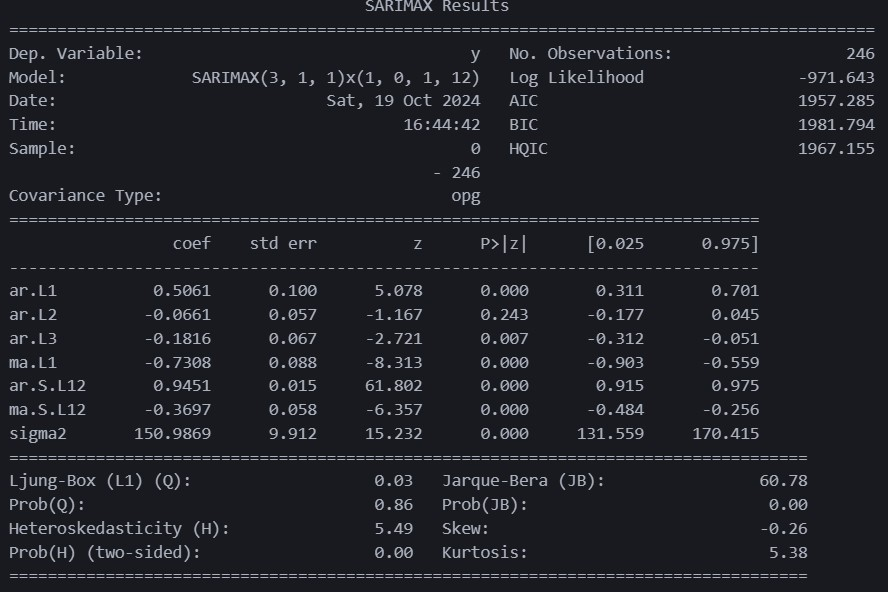
\includegraphics[scale=0.85]{images/sarimax_results_pt4_q1.jpg}
\caption{Tabela de resultados - SARIMA}
\end{figure}

\subsubsection{(a) Quantos modelos foram comparados para selecionar o modelo sub-ótimo?}

O procedimento \texttt{auto\_arima} comparou \textbf{87 modelos} durante a busca stepwise, considerando várias combinações de valores para \(p\), \(q\), \(P\), \(Q\) e incluindo sazonalidade com \(m=12\). O melhor modelo selecionado foi o \textbf{SARIMA(3,1,1)(1,0,1)$_{12}$}, que minimizou o critério AICc, tornando-se o modelo sub-ótimo.

\subsubsection{(b) AICc e a equação SARIMA(p,d,q)(P,D,Q) em termos das ordens p, q, d, D, P e Q }

O melhor modelo SARIMA selecionado foi o \textbf{SARIMA(3,1,1)(1,0,1)$_{12}$}, que inclui tanto componentes não-sazonais quanto componentes sazonais com período \(m=12\). A tabela com os parâmetros do modelo foi gerada pelo procedimento \texttt{auto\_arima} e está resumida a seguir:

\begin{itemize}
    \item \(p = 3\): três termos autorregressivos não-sazonais;
    \item \(d = 1\): uma diferenciação não-sazonal;
    \item \(q = 1\): um termo de média móvel não-sazonal;
    \item \(P = 1\): um termo autorregressivo sazonal com período \(m=12\);
    \item \(D = 0\): nenhuma diferenciação sazonal;
    \item \(Q = 1\): um termo de média móvel sazonal com período \(m=12\).
\end{itemize}

O valor do critério de informação AICc para esse modelo foi 1957.756. Esse critério sugere que o modelo é o mais parcimonioso entre os testados, balanceando ajuste e simplicidade.

A equação SARIMA correspondente ao modelo ajustado é:

\[
(1 - 0.5061 L + 0.0661 L^2 + 0.1816 L^3)(1 - L) y_t = (1 - 0.7308 L)(1 - 0.9451 L^{12} + 0.3697 L^{12}) \epsilon_t
\]

Onde:
\begin{itemize}
    \item \(y_t\) é a série temporal original;
    \item \(L\) é o operador de defasagem;
    \item \(\epsilon_t\) é o erro aleatório (ruído branco).
\end{itemize}

\subsubsection{(c)  FAC e FACP dos resíduos e o resultado do teste Ljung-Box para \(m=20\)}

Após o ajuste do modelo, analisamos a Função de Autocorrelação (FAC) e a Função de Autocorrelação Parcial (FACP) dos resíduos para verificar a presença de padrões de dependência não capturados pelo modelo. Além disso, realizamos o teste de Ljung-Box com \(m=20\), que testa a hipótese de que não há autocorrelação significativa até a defasagem 20.

O código para gerar os gráficos da FAC e FACP e realizar o teste de Ljung-Box é mostrado a seguir:

\begin{lstlisting}[style=python]
# Obter os resíduos do modelo ajustado
residuals_sarima = model_sarima.resid()

# Plotar a FAC e FACP dos resíduos
plt.figure(figsize=(12, 6))

# FAC dos resíduos
plt.subplot(1, 2, 1)
plot_acf(residuals_sarima, lags=36, ax=plt.gca(),
         title='FAC dos Resíduos (SARIMA)')

# FACP dos resíduos
plt.subplot(1, 2, 2)
plot_pacf(residuals_sarima, lags=36, ax=plt.gca(),
          title='FACP dos Resíduos (SARIMA)')

plt.tight_layout()
plt.show()

# Teste de Ljung-Box para m=20
ljung_box_results = acorr_ljungbox(residuals_sarima, lags=[20], return_df=True)
print(ljung_box_results)
\end{lstlisting}

\subsubsection*{FAC e FACP dos Resíduos}

Os gráficos da Função de Autocorrelação (FAC) e da Função de Autocorrelação Parcial (FACP) dos resíduos são mostrados abaixo:

\begin{figure}[H]
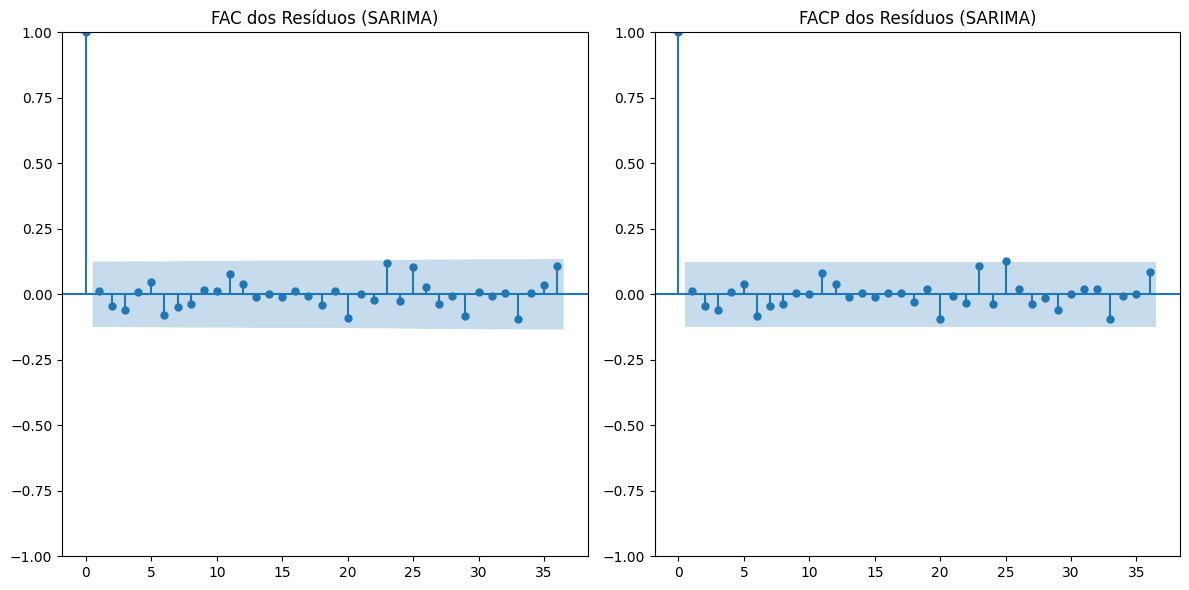
\includegraphics[scale=0.5]{images/fac_facp_1_iv_c.png}
\caption{Gráficos da FAC e da FACP dos resíduos do modelo SARIMA(3,1,1)(1,0,1)$_{12}$}
\end{figure}

\begin{itemize}
    \item A \textbf{FAC dos resíduos} mostra que os resíduos do modelo estão dentro dos limites de confiança para todas as defasagens, sugerindo que o modelo capturou adequadamente a estrutura de dependência da série temporal.
    \item A \textbf{FACP dos resíduos} confirma essa análise, já que nenhum lag mostra correlação significativa.
\end{itemize}

\subsubsection*{Resultado do Teste de Ljung-Box para \(m=20\)}

O teste de Ljung-Box foi aplicado para verificar a independência dos resíduos até a defasagem \(m=20\), e os resultados foram os seguintes:

\[
\text{Estatística Ljung-Box} = 9.26935, \quad \text{p-valor} = 0.979572
\] \\

Como o p-valor é significativamente maior que 0.05, não podemos rejeitar a hipótese nula de que os resíduos são independentes. Isso indica que não há autocorrelação significativa nos resíduos do modelo SARIMA(3,1,1)(1,0,1)$_{12}$, sugerindo que o modelo é adequado e os resíduos se comportam como ruído branco.

Com base nesses resultados, concluímos que o modelo sub-ótimo SARIMA(3,1,1)(1,0,1)$_{12}$ é eficaz para capturar a estrutura da série temporal, não deixando padrões de dependência não explicados nos resíduos.\\\\

\subsection{Questão 1: Parte (v)}
\textbf{Sabemos que as funções de ajuste automático do SARIMA geralmente realizam uma busca
“econômica” para poupar recursos computacionais. Agora queremos que vc realize uma busca
mais extensa para chegar ao melhor modelo SARIMA para a sua série (denomine esse modelo
de ótimo).}\\

Nesta primeira etapa, podemos utilizar o \textit{auto\_arima} com uma busca mais extensa, removendo a opção de busca "\textit{stepwise}", que é mais econômica computacionalmente. Isso permitirá que o algoritmo teste um número maior de combinações de parâmetros.\\

O código foi ajustado da seguinte forma:\\

\begin{lstlisting} [style=python]
# Ajustar o modelo SARIMA com uma busca mais extensa (sem stepwise)
model_sarima_extenso = pm.auto_arima(train['Vendas'],
                     start_p=0, max_p=5,
                     start_q=0, max_q=5,
                     d=None, D=None,   #Permitir que o modelo escolha d e D
                     seasonal=True,   #Habilitar sazonalidade
                     # Periodo sazonal (12 meses)
                     m=12,
                     information_criterion='aicc',
                     trace=True,
                     stepwise=False)   #Desabilitar busca stepwise

# Exibir o resumo do modelo
print(model_sarima_extenso.summary())

# Valor de AICc
aicc_value_extenso = model_sarima_extenso.aicc()
print(f"Valor do AICc: {aicc_value_extenso}")
\end{lstlisting}

\begin{verbatim}
 ARIMA(0,1,0)(0,0,0)[12] intercept   : AICC=2388.242, Time=0.02 sec
 ARIMA(0,1,0)(0,0,1)[12] intercept   : AICC=2211.816, Time=0.17 sec
 ARIMA(0,1,0)(0,0,2)[12] intercept   : AICC=2154.849, Time=0.31 sec
 ARIMA(0,1,0)(1,0,0)[12] intercept   : AICC=2014.213, Time=0.17 sec
 ARIMA(0,1,0)(1,0,1)[12] intercept   : AICC=1987.874, Time=0.25 sec
 ARIMA(0,1,0)(1,0,2)[12] intercept   : AICC=1989.777, Time=0.87 sec
 ARIMA(0,1,0)(2,0,0)[12] intercept   : AICC=inf, Time=0.61 sec
 ARIMA(0,1,0)(2,0,1)[12] intercept   : AICC=1989.862, Time=0.66 sec
 ARIMA(0,1,0)(2,0,2)[12] intercept   : AICC=inf, Time=3.47 sec
 ARIMA(0,1,1)(0,0,0)[12] intercept   : AICC=2357.891, Time=0.07 sec
 ARIMA(0,1,1)(0,0,1)[12] intercept   : AICC=2198.753, Time=0.16 sec
 ARIMA(0,1,1)(0,0,2)[12] intercept   : AICC=2153.700, Time=0.50 sec
 ARIMA(0,1,1)(1,0,0)[12] intercept   : AICC=2013.866, Time=0.21 sec
 ARIMA(0,1,1)(1,0,1)[12] intercept   : AICC=1986.478, Time=0.31 sec
 ARIMA(0,1,1)(1,0,2)[12] intercept   : AICC=1987.732, Time=0.81 sec
 ARIMA(0,1,1)(2,0,0)[12] intercept   : AICC=1990.705, Time=0.58 sec
 ARIMA(0,1,1)(2,0,1)[12] intercept   : AICC=1988.166, Time=0.70 sec
 ARIMA(0,1,1)(2,0,2)[12] intercept   : AICC=1985.975, Time=1.71 sec
 ARIMA(0,1,2)(0,0,0)[12] intercept   : AICC=2340.579, Time=0.09 sec
 ARIMA(0,1,2)(0,0,1)[12] intercept   : AICC=2185.960, Time=0.22 sec
 ARIMA(0,1,2)(0,0,2)[12] intercept   : AICC=2136.121, Time=0.74 sec
 ARIMA(0,1,2)(1,0,0)[12] intercept   : AICC=1999.933, Time=0.32 sec
 ARIMA(0,1,2)(1,0,1)[12] intercept   : AICC=1974.432, Time=0.42 sec
 ARIMA(0,1,2)(1,0,2)[12] intercept   : AICC=1975.738, Time=1.80 sec
 ARIMA(0,1,2)(2,0,0)[12] intercept   : AICC=1977.315, Time=1.59 sec
 ARIMA(0,1,2)(2,0,1)[12] intercept   : AICC=1976.081, Time=0.98 sec
 ARIMA(0,1,3)(0,0,0)[12] intercept   : AICC=2305.408, Time=0.38 sec
 ARIMA(0,1,3)(0,0,1)[12] intercept   : AICC=2149.221, Time=0.34 sec
 ARIMA(0,1,3)(0,0,2)[12] intercept   : AICC=2095.536, Time=1.47 sec
 ARIMA(0,1,3)(1,0,0)[12] intercept   : AICC=1975.217, Time=0.31 sec
 ARIMA(0,1,3)(1,0,1)[12] intercept   : AICC=1954.929, Time=0.56 sec
 ARIMA(0,1,3)(2,0,0)[12] intercept   : AICC=1959.068, Time=0.86 sec
 ARIMA(0,1,4)(0,0,0)[12] intercept   : AICC=2293.762, Time=0.14 sec
 ARIMA(0,1,4)(0,0,1)[12] intercept   : AICC=2140.649, Time=0.50 sec
 ARIMA(0,1,4)(1,0,0)[12] intercept   : AICC=1976.517, Time=0.71 sec
 ARIMA(0,1,5)(0,0,0)[12] intercept   : AICC=2282.101, Time=0.46 sec
 ARIMA(1,1,0)(0,0,0)[12] intercept   : AICC=2370.930, Time=0.04 sec
 ARIMA(1,1,0)(0,0,1)[12] intercept   : AICC=2203.781, Time=0.25 sec
 ARIMA(1,1,0)(0,0,2)[12] intercept   : AICC=2154.665, Time=0.74 sec
 ARIMA(1,1,0)(1,0,0)[12] intercept   : AICC=2014.585, Time=0.23 sec
 ARIMA(1,1,0)(1,0,1)[12] intercept   : AICC=1987.505, Time=0.32 sec
 ARIMA(1,1,0)(1,0,2)[12] intercept   : AICC=1989.037, Time=1.02 sec
 ARIMA(1,1,0)(2,0,0)[12] intercept   : AICC=inf, Time=0.61 sec
 ARIMA(1,1,0)(2,0,1)[12] intercept   : AICC=1989.322, Time=0.68 sec
 ARIMA(1,1,0)(2,0,2)[12] intercept   : AICC=1987.629, Time=1.26 sec
 ARIMA(1,1,1)(0,0,0)[12] intercept   : AICC=2358.460, Time=0.12 sec
 ARIMA(1,1,1)(0,0,1)[12] intercept   : AICC=2200.250, Time=0.45 sec
 ARIMA(1,1,1)(0,0,2)[12] intercept   : AICC=2153.279, Time=1.03 sec
 ARIMA(1,1,1)(1,0,0)[12] intercept   : AICC=1986.187, Time=0.83 sec
 ARIMA(1,1,1)(1,0,1)[12] intercept   : AICC=1964.460, Time=0.52 sec
 ARIMA(1,1,1)(1,0,2)[12] intercept   : AICC=1966.323, Time=1.17 sec
 ARIMA(1,1,1)(2,0,0)[12] intercept   : AICC=1968.207, Time=0.97 sec
 ARIMA(1,1,1)(2,0,1)[12] intercept   : AICC=1966.437, Time=1.50 sec
 ARIMA(1,1,2)(0,0,0)[12] intercept   : AICC=2312.557, Time=0.11 sec
 ARIMA(1,1,2)(0,0,1)[12] intercept   : AICC=2156.005, Time=0.35 sec
 ARIMA(1,1,2)(0,0,2)[12] intercept   : AICC=2110.999, Time=0.99 sec
 ARIMA(1,1,2)(1,0,0)[12] intercept   : AICC=1986.047, Time=0.54 sec
 ARIMA(1,1,2)(1,0,1)[12] intercept   : AICC=1964.553, Time=0.52 sec
 ARIMA(1,1,2)(2,0,0)[12] intercept   : AICC=1968.570, Time=2.08 sec
 ARIMA(1,1,3)(0,0,0)[12] intercept   : AICC=2304.092, Time=0.10 sec
 ARIMA(1,1,3)(0,0,1)[12] intercept   : AICC=2146.297, Time=0.36 sec
 ARIMA(1,1,3)(1,0,0)[12] intercept   : AICC=1976.825, Time=0.31 sec
 ARIMA(1,1,4)(0,0,0)[12] intercept   : AICC=2290.804, Time=0.47 sec
 ARIMA(2,1,0)(0,0,0)[12] intercept   : AICC=2338.949, Time=0.06 sec
 ARIMA(2,1,0)(0,0,1)[12] intercept   : AICC=2186.890, Time=0.21 sec
 ARIMA(2,1,0)(0,0,2)[12] intercept   : AICC=2147.087, Time=0.95 sec
 ARIMA(2,1,0)(1,0,0)[12] intercept   : AICC=2013.674, Time=0.35 sec
 ARIMA(2,1,0)(1,0,1)[12] intercept   : AICC=1986.706, Time=0.38 sec
 ARIMA(2,1,0)(1,0,2)[12] intercept   : AICC=1988.246, Time=0.86 sec
 ARIMA(2,1,0)(2,0,0)[12] intercept   : AICC=inf, Time=0.69 sec
 ARIMA(2,1,0)(2,0,1)[12] intercept   : AICC=1988.519, Time=1.04 sec
 ARIMA(2,1,1)(0,0,0)[12] intercept   : AICC=2293.048, Time=0.11 sec
 ARIMA(2,1,1)(0,0,1)[12] intercept   : AICC=2140.833, Time=0.48 sec
 ARIMA(2,1,1)(0,0,2)[12] intercept   : AICC=2099.504, Time=1.53 sec
 ARIMA(2,1,1)(1,0,0)[12] intercept   : AICC=1984.878, Time=0.61 sec
 ARIMA(2,1,1)(1,0,1)[12] intercept   : AICC=1963.375, Time=0.49 sec
 ARIMA(2,1,1)(2,0,0)[12] intercept   : AICC=1967.545, Time=1.72 sec
 ARIMA(2,1,2)(0,0,0)[12] intercept   : AICC=2295.125, Time=0.14 sec
 ARIMA(2,1,2)(0,0,1)[12] intercept   : AICC=2142.586, Time=0.47 sec
 ARIMA(2,1,2)(1,0,0)[12] intercept   : AICC=1985.792, Time=0.82 sec
 ARIMA(2,1,3)(0,0,0)[12] intercept   : AICC=2296.832, Time=0.26 sec
 ARIMA(3,1,0)(0,0,0)[12] intercept   : AICC=2325.354, Time=0.12 sec
 ARIMA(3,1,0)(0,0,1)[12] intercept   : AICC=2167.358, Time=0.23 sec
 ARIMA(3,1,0)(0,0,2)[12] intercept   : AICC=2119.265, Time=0.56 sec
 ARIMA(3,1,0)(1,0,0)[12] intercept   : AICC=1989.856, Time=0.33 sec
 ARIMA(3,1,0)(1,0,1)[12] intercept   : AICC=1967.095, Time=0.47 sec
 ARIMA(3,1,0)(2,0,0)[12] intercept   : AICC=inf, Time=0.79 sec
 ARIMA(3,1,1)(0,0,0)[12] intercept   : AICC=2295.125, Time=0.22 sec
 ARIMA(3,1,1)(0,0,1)[12] intercept   : AICC=2142.482, Time=0.53 sec
 ARIMA(3,1,1)(1,0,0)[12] intercept   : AICC=1981.857, Time=0.60 sec
 ARIMA(3,1,2)(0,0,0)[12] intercept   : AICC=2294.938, Time=0.23 sec
 ARIMA(4,1,0)(0,0,0)[12] intercept   : AICC=2324.469, Time=0.11 sec
 ARIMA(4,1,0)(0,0,1)[12] intercept   : AICC=2165.654, Time=0.26 sec
 ARIMA(4,1,0)(1,0,0)[12] intercept   : AICC=1986.796, Time=0.47 sec
 ARIMA(4,1,1)(0,0,0)[12] intercept   : AICC=2318.835, Time=0.26 sec
 ARIMA(5,1,0)(0,0,0)[12] intercept   : AICC=2326.554, Time=0.23 sec

Best model:  ARIMA(0,1,3)(1,0,1)[12] intercept
Total fit time: 57.652 seconds
\end{verbatim}

\begin{figure}[H]
\centering
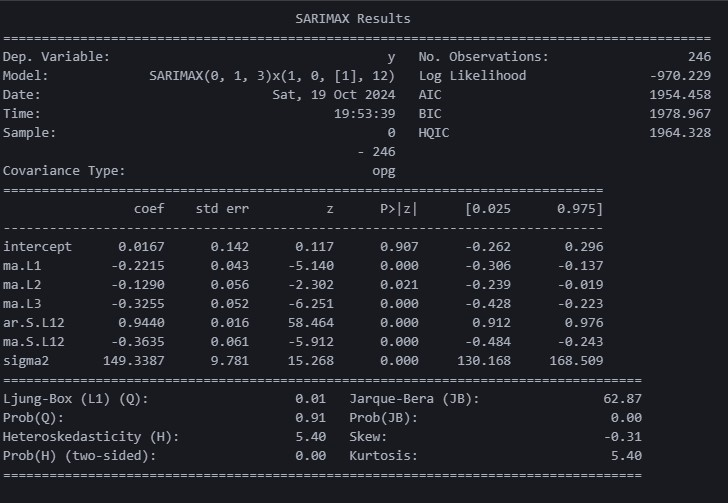
\includegraphics[scale=0.98]{images/sarima_results_extenso.jpg}
\caption{Tabela  de resultados: execução extensa - SARIMA}
\end{figure}

\subsubsection{(a) Contrastando o número de modelos que foram comparados na busca do modelo ótimo com
aquele obtido na busca do modelo sub-ótimo efetuada em (iv)}

A busca sub-ótima realizada na parte (iv) utilizou o parâmetro \textit{stepwise=True}, o que restringe o número de modelos comparados para otimizar o tempo computacional. Naquela busca, foram comparados 87 modelos.

Na busca ótima atual, ao removermos o \textit{stepwise}, o número de combinações testadas aumentou significativamente. Nesse caso, foram comparados 96 modelos. A diferença é justificada pela remoção da busca restrita, permitindo um exame mais profundo de combinações de parâmetros.

\begin{itemize}
    \item \textbf{Busca Sub-ótima (iv)}: 87 modelos comparados.
    \item \textbf{Busca Ótima (v)}: 96 modelos comparados.
\end{itemize}

\subsubsection{(b) AICc e Expressão dos Modelos}

O melhor modelo encontrado na busca ótima foi o \textbf{SARIMA(0,1,3)(1,0,1)$_{12}$}, conforme o resultado da parte (v). O valor de AICc para este modelo foi \textbf{1954.93}. O segundo melhor modelo foi o \textbf{SARIMA(3,1,1)(1,0,1)$_{12}$}, obtido na parte (iv), com um AICc de \textbf{1957.76}. Para cada um dos dois modelos, vamos descrever as três expressões requisitadas: a especificação em termos dos operadores de atraso \( L \) e \( L^{12} \), a expressão em termos de \( y_t \) e \( \epsilon_t \), e as ordens \( p, q, d, P, D, Q \).\\

\textbf{Melhor modelo: SARIMA(0,1,3)(1,0,1)$_{12}$}

\begin{itemize}
    \item \( p = 0 \): Não há termos autorregressivos não sazonais.
    \item \( d = 1 \): Uma diferenciação não sazonal.
    \item \( q = 3 \): Três termos de média móvel não sazonais.
    \item \( P = 1 \): Um termo autorregressivo sazonal com período 12.
    \item \( D = 0 \): Nenhuma diferenciação sazonal.
    \item \( Q = 1 \): Um termo de média móvel sazonal com período 12.
\end{itemize}

A equação SARIMA correspondente ao melhor modelo é expressa em três formas:

\begin{enumerate}
    \item \textbf{Operadores de atraso em termos de \( L \) e \( L^{12} \):}
    \[
    (1 - \theta_1 L - \theta_2 L^2 - \theta_3 L^3)(1 - L) y_t = (1 - \Theta_1 L^{12})(1 - \Psi_1 L^{12}) \epsilon_t
    \]
    
    \item \textbf{Expressão em termos de valores defasados de \( y_t \) e \( \epsilon_t \):}
    \[
    y_t - y_{t-1} = -\theta_1 \epsilon_{t-1} - \theta_2 \epsilon_{t-2} - \theta_3 \epsilon_{t-3} + \epsilon_t + \Theta_1 \epsilon_{t-12} + \Psi_1 \epsilon_{t-12}
    \]

    \item \textbf{Valores numéricos dos parâmetros ajustados:}
    \[
    y_t - y_{t-1} = -0.2215 \epsilon_{t-1} - 0.1299 \epsilon_{t-2} - 0.3255 \epsilon_{t-3} + \epsilon_t + 0.9440 \epsilon_{t-12} - 0.3635 \epsilon_{t-12}
    \]
\end{enumerate}

\textbf{Segundo melhor modelo: SARIMA(3,1,1)(1,0,1)$_{12}$}

\begin{itemize}
    \item \( p = 3 \): Três termos autorregressivos não sazonais.
    \item \( d = 1 \): Uma diferenciação não sazonal.
    \item \( q = 1 \): Um termo de média móvel não sazonal.
    \item \( P = 1 \): Um termo autorregressivo sazonal com período 12.
    \item \( D = 0 \): Nenhuma diferenciação sazonal.
    \item \( Q = 1 \): Um termo de média móvel sazonal com período 12.
\end{itemize}

A equação SARIMA correspondente ao segundo melhor modelo é expressa em três formas:

\begin{enumerate}
    \item \textbf{Operadores de atraso em termos de \( L \) e \( L^{12} \):}
    \[
    (1 - \phi_1 L - \phi_2 L^2 - \phi_3 L^3)(1 - L) y_t = (1 - \Theta_1 L^{12})(1 - \Psi_1 L^{12}) \epsilon_t
    \]
    
    \item \textbf{Expressão em termos de valores defasados de \( y_t \) e \( \epsilon_t \):}
    \[
    y_t - y_{t-1} = \phi_1 y_{t-1} + \phi_2 y_{t-2} + \phi_3 y_{t-3} - \theta_1 \epsilon_{t-1} + \epsilon_t + \Theta_1 \epsilon_{t-12} + \Psi_1 \epsilon_{t-12}
    \]

    \item \textbf{Valores numéricos dos parâmetros ajustados:}
    \[
    y_t - y_{t-1} = 0.5061 y_{t-1} + 0.0661 y_{t-2} + 0.1816 y_{t-3} - 0.7308 \epsilon_{t-1} + \epsilon_t + 0.9451 \epsilon_{t-12} - 0.3697 \epsilon_{t-12}
    \]
\end{enumerate}

O modelo \textbf{SARIMA(0,1,3)(1,0,1)$_{12}$} apresentou um AICc menor, indicando que captura melhor a estrutura temporal da série de vendas do que o modelo \textbf{SARIMA(3,1,1)(1,0,1)$_{12}$}. A principal diferença está nas ordens de \( p \) e \( q \), que são diferentes entre os modelos. No entanto, ambos os modelos capturam adequadamente as componentes sazonais e não sazonais, sendo adequados para prever a série temporal.


\subsubsection{(c) FAC/FACP dos resíduos e o resultado do teste Ljung-Box para m=20}

Após ajustar o modelo, analisamos os resíduos para verificar a adequação do ajuste.

\begin{lstlisting} [style=python]
# Obter os resíduos do modelo ajustado
residuals_sarima_extenso = model_sarima_extenso.resid()

# Plotar a FAC e FACP dos residuos
plt.figure(figsize=(12, 6))

# FAC dos residuos
plt.subplot(1, 2, 1)
plot_acf(residuals_sarima_extenso, lags=36, ax=plt.gca(),
         title='FAC dos Residuos (SARIMA)')

# FACP dos residuos
plt.subplot(1, 2, 2)
plot_pacf(residuals_sarima_extenso, lags=36, ax=plt.gca(),
          title='FACP dos Residuos (SARIMA)')

plt.tight_layout()
plt.show()

# Teste de Ljung-Box para m=20
ljung_box_results_extenso = acorr_ljungbox(residuals_sarima_extenso, lags=[20], return_df=True)
print(ljung_box_results_extenso)
\end{lstlisting}

\begin{figure}[H]
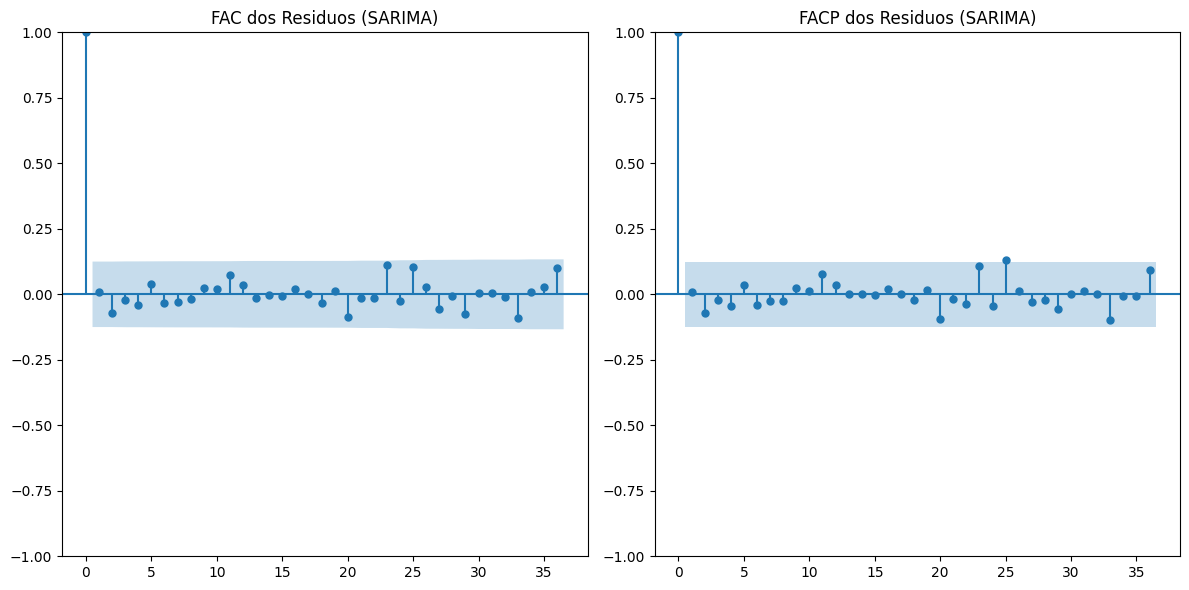
\includegraphics[scale=0.5]{images/fac_facp_Extenso.png}
\caption{Gráficos da FAC e FACP dos resíduos do modelo ótimo obtido}
\end{figure}

Os resultados da FAC e FACP dos resíduos indicam que não há autocorrelações significativas restantes nos resíduos, confirmando que o modelo SARIMA capturou bem as dependências temporais da série. Além disso, o teste de Ljung-Box para \(m = 20\) não rejeita a hipótese nula de independência dos resíduos (\(p = 0.99\)), o que também sugere que os resíduos se comportam como ruído branco.

\begin{itemize}
    \item \textbf{Estatística do Teste de Ljung-Box (m=20)}: 7.27
    \item \textbf{p-valor}: 0.9957
\end{itemize}

Com base no teste de Ljung-Box e nos gráficos de FAC e FACP, o modelo ótimo ajustado é considerado adequado, uma vez que os resíduos são independentes e seguem um comportamento de ruído branco.\\\\




\subsection{Questão 1: Parte (vi)}
\textbf{A partir dos resultados dos 3 modelos SARIMA ajustados: o não-sazonal, o sub-ótimo e o ótimo, obter:}

\subsubsection{(a) A Expressão SARIMA(p,d,q)(P,D,Q) de Cada Modelo}

As expressões SARIMA para cada modelo ajustado são as seguintes:

\begin{itemize}
    \item \textbf{Modelo Não-Sazonal: SARIMA(2,1,1)(0,0,0)[0]}
    
    A equação autorregressiva não-sazonal com média móvel é dada por:
    \[
    (1 - 1.0383L + 0.5265L^2)(1 - L)y_t = (1 - 0.8866L)\epsilon_t
    \]
    Onde \(L\) é o operador de defasagem (lag) e \(y_t\) é a série temporal. 

    \item \textbf{Modelo Sub-Ótimo: SARIMA(3,1,1)(1,0,1)[12]}
    
    Este modelo inclui componentes sazonais e não-sazonais. A equação autorregressiva e de média móvel é:
    \[
    (1 - 0.5061L + 0.0661L^2 + 0.1816L^3)(1 - L)y_t = (1 - 0.7308L)(1 - 0.9451L^{12} + 0.3697L^{12})\epsilon_t
    \]
    Onde \(L^{12}\) representa o operador de defasagem sazonal com período 12 (mensal).
    
    \item \textbf{Modelo Ótimo: SARIMA(0,1,3)(1,0,1)[12]}
    
    A equação de média móvel e de autorregressão sazonal é:
    \[
    (1 - L)y_t = (1 - 0.2215L - 0.1299L^2 - 0.3255L^3)(1 - 0.9440L^{12} + 0.3635L^{12})\epsilon_t
    \]
\end{itemize}

As expressões acima apresentam as componentes não-sazonais e sazonais de cada modelo, juntamente com os operadores de defasagem aplicados à série \(y_t\) e ao termo de erro \(\epsilon_t\).





\subsubsection{(b) O Valor do AICc de Cada Modelo}

Abaixo apresentamos os valores do Critério de Informação de Akaike corrigido (AICc) para os três modelos ajustados. Separamos uma parte no código para enfatizar os resultados.

\begin{lstlisting}[style=python]
""" Parte vi"""
"""(b)"""

# Valor de AICc - modelo sazonal
aicc_value_modeloSazonal = modeliii.aicc()
print(f"Valor do AICc do modelo sazonal: {aicc_value_modeloSazonal}")

# Valor de AICc - modelo sub-otimo
aicc_value_modeloSubOtimo = model_sarima.aicc()
print(f"Valor do AICc do modelo sub-otimo: {aicc_value_modeloSubOtimo}")

# Valor de AICc - modelo otimo
aicc_value_modeloOtimo = model_sarima_extenso.aicc()
print(f"Valor do AICc do modelo otimo: {aicc_value_modeloOtimo}")

\end{lstlisting}

\begin{figure}[H]
\centering
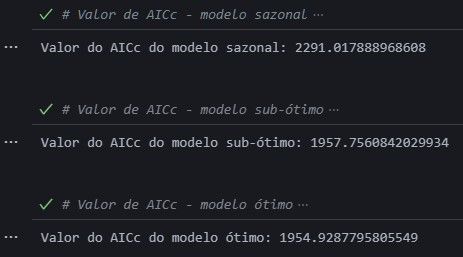
\includegraphics[scale=1.2]{images/letraB_parteVI.jpg}
\caption{Saída do Programa: Valor do AICc de cada modelo}
\end{figure}

\begin{table}[H]
\centering
\caption{Valores do AICc dos Modelos Ajustados}
\begin{tabular}{|c|c|}
\hline
\textbf{Modelo}          & \textbf{AICc} \\ \hline
Não-Sazonal   & 2291.0179 \\ \hline
Sub-Ótimo     & 1957.7561 \\ \hline
Ótimo         & 1954.9288 \\ \hline
\end{tabular}
\end{table}

\noindent Como podemos observar na tabela acima, o valor do AICc do modelo não-sazonal é significativamente maior em comparação com os modelos que incorporam a sazonalidade, indicando um ajuste menos eficiente. O modelo que apresenta o menor valor de AICc é o modelo \textit{ótimo} (1954.9288), sugerindo que esse é o modelo mais adequado entre os três para capturar a estrutura da série temporal.

\subsubsection{(c) Valores dos coeficientes de autocorrelação dos resíduos e teste Ljung-Box para m=20}

Para enfatizar esta parte, separamos um trecho de código para evidenciar os resultados:

\begin{lstlisting}[style=python]
"""(c)"""
lags = [1, 2, 3, 6, 12]


""" Modelo sazonal"""
acf_values_seasonal = sm.tsa.acf(residuals_modeliii, nlags=max(lags))

# Criar um DataFrame para exibir os valores de autocorrelacao para os lags desejados
acf_lags_seasonal = pd.DataFrame({'Lag': lags, 'ACF': acf_values_seasonal[lags]})

print(acf_lags_seasonal)

# Realizar o teste Ljung-Box para m=20
ljung_box_results_seasonal = sm.stats.acorr_ljungbox(
    residuals_modeliii, lags=[20], return_df=True)
print(ljung_box_results_seasonal)


""" Modelo sub-otimo"""
acf_values_subOtimo = sm.tsa.acf(residuals_sarima, nlags=max(lags))

# Criar um DataFrame para exibir os valores de autocorrelacao para os lags desejados
acf_lags_subOtimo = pd.DataFrame({'Lag': lags, 'ACF': acf_values_subOtimo[lags]})

print(acf_lags_subOtimo)

# Realizar o teste Ljung-Box para m=20
ljung_box_results = sm.stats.acorr_ljungbox(
    residuals_sarima, lags=[20], return_df=True)
print(ljung_box_results)



""" Modelo otimo"""
acf_values = sm.tsa.acf(residuals_sarima_extenso, nlags=max(lags))

# Criar um DataFrame para exibir os valores de autocorrelacao para os lags desejados
acf_lags = pd.DataFrame({'Lag': lags, 'ACF': acf_values[lags]})

print(acf_lags)

# Realizar o teste Ljung-Box para m=20
ljung_box_results = sm.stats.acorr_ljungbox(
    residuals_sarima_extenso, lags=[20], return_df=True)
print(ljung_box_results)

\end{lstlisting}

\begin{figure}[H]
\centering
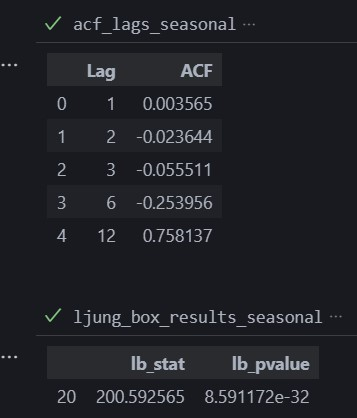
\includegraphics[scale=0.9]{images/vi_c_sazonal.jpg}
\caption{Saída do Programa: coeficientes de autocorrelação e Ljung-Box para o modelo sazonal}
\end{figure}

\begin{figure}[H]
\centering
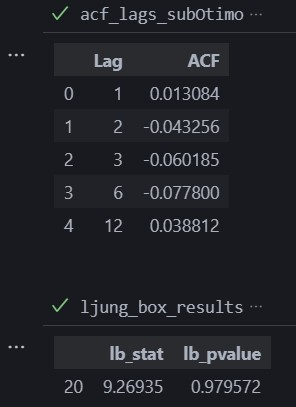
\includegraphics[scale=0.9]{images/vi_c_subotimo.jpg}
\caption{Saída do Programa: coeficientes de autocorrelação e Ljung-Box para o modelo sub-ótimo}
\end{figure}

\begin{figure}[H]
\centering
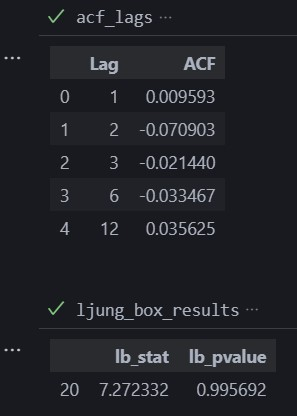
\includegraphics[scale=0.9]{images/vi_c_otimo.jpg}
\caption{Saída do Programa: coeficientes de autocorrelação e Ljung-Box para o modelo ótimo}
\end{figure}

Abaixo estão apresentados, de forma organizada, os valores dos coeficientes de autocorrelação dos resíduos nos lags 1, 2, 3, 6 e 12, assim como os resultados do teste Ljung-Box para \(m=20\), para cada um dos três modelos ajustados.

\begin{table}[H]
\centering
\caption{Coeficientes de Autocorrelação dos Resíduos e Teste Ljung-Box}
\begin{tabular}{|c|c|c|c|c|c|c|c|}
\hline
\textbf{Modelo} & \textbf{Lag 1} & \textbf{Lag 2} & \textbf{Lag 3} & \textbf{Lag 6} & \textbf{Lag 12} & \textbf{Ljung-Box Q-stat} & \textbf{p-valor} \\ \hline
Não-Sazonal   & 0.0036  & -0.0236 & -0.055 & -0.254  & 0.758 & 200.59  & 8.59e-32  \\ \hline
Sub-Ótimo     & 0.013 & -0.043  & -0.060 & -0.078  & 0.0389 & 9.27  & 0.98   \\ \hline
Ótimo         & 0.0096  & -0.071  & -0.021 & -0.033  & 0.036 & 7.27  & 0.995 \\ \hline
\end{tabular}
\end{table}

\noindent  Analisando os coeficientes de autocorrelação dos resíduos e os resultados do teste Ljung-Box para os três modelos:

\begin{itemize}
    \item \textbf{Modelo Não-Sazonal:}  O modelo não-sazonal apresenta coeficientes de autocorrelação mistos. Embora tenha o menor valor de autocorrelação no Lag 6 (-0.254), no Lag 12 ele apresenta o maior valor (0.758), o que indica uma possível falha na captura da sazonalidade, mesmo com o p-valor do Ljung-Box sendo muito baixo (8.59e-32). Isso sugere que este modelo não consegue remover completamente as dependências temporais nos resíduos, especialmente no componente sazonal, resultando em resíduos que apresentam sinais de autocorrelação significativa.
    \item \textbf{Modelo Sub-Ótimo:} O modelo sub-ótimo tem desempenho interessante nos primeiros lags, com o maior valor de autocorrelação no Lag 1 (0.013), mas ele apresenta o menor valor no Lag 3 (-0.060). No geral, seus coeficientes são mais estáveis e próximos de zero, especialmente no Lag 12 (0.0389), o que é um sinal positivo. O p-valor do teste Ljung-Box (0.98) sugere que este modelo captura bem a estrutura da série, produzindo resíduos que se aproximam de ruído branco. Ainda assim, a pequena autocorrelação no Lag 1 e os valores flutuantes indicam que ele pode não ser tão eficiente quanto o modelo ótimo.

    \item \textbf{Modelo Ótimo:} Este modelo apresenta o menor valor de autocorrelação no Lag 12 (0.036), o que mostra que ele lida bem com a sazonalidade, mas não tem os menores valores em todos os lags. No Lag 1, por exemplo, ele tem um valor maior que o modelo não-sazonal, mas menor que o sub-ótimo. No Lag 3, seu valor é o maior (-0.021), o que pode indicar alguma dificuldade na captura de dependências em curtos prazos. Apesar dessas flutuações, o p-valor muito alto do teste Ljung-Box (0.995) sugere que os resíduos desse modelo são praticamente independentes e próximos de ruído branco, o que o torna o mais robusto entre os três.
    
    
\end{itemize}

Com base nesses resultados, o \textbf{modelo ótimo} é a melhor escolha, pois, embora não apresente os menores coeficientes em todos os lags, ele captura bem a sazonalidade, apresenta o menor valor de AICc e os resíduos mais próximos de ruído branco, com um p-valor de Ljung-Box indicando forte independência nos resíduos.\\\\

\section{Questão 2}

Agora, devemos considerar o \textbf{período de teste} da série. Para os 3 modelos (não-sazonal, sub-ótimo e ótimo), incluindo o melhor modelo ETS obtido no trabalho 01, \textbf{ETS(A,Ad,A)}, bem como os métodos ingênuos de previsão:

\begin{itemize}
    \item \textbf{método ing. 1}: a previsão em qualquer horizonte $h$ é igual à última observação da ST no período de treinamento;
    \item \textbf{método ing. 2}: a previsão em qualquer horizonte $h$ é igual ao valor da última observação da série, no período de treinamento, correspondente aquele mês que está sendo previsto no período de teste.
\end{itemize}

Devemos obter uma tabela comparativa contendo:

\begin{itemize}
    \item Valor da série;
    \item Previsão k-passos à frente de cada modelo/método, $k=1,2,...12$;
    \item Medidas de aderência (RMSE, MAD, MAPE, SMape, MASE);
\end{itemize}

Vamos desenvolver esta questão passo-a-passo por tópicos.

\subsection{Obtendo as Previsões}

Para cada um dos 3 modelos SARIMA (não-sazonal, sub-ótimo e ótimo) e o modelo ETS(A,Ad,A), devemos calcular as previsões para os 12 próximos períodos de teste.\\

\begin{lstlisting}[style=python]
""" *** QUESTAO 2 *** """

h = len(test) #numero de passos a frente

# Previsões para o modelo não-sazonal
forecast_nao_sazonal = modeliii.predict(n_periods=h)

# Previsões para o modelo sub-otimo
forecast_sub_otimo = model_sarima.predict(n_periods=h)

# Previsões para o modelo otimo
forecast_otimo = model_sarima_extenso.predict(n_periods=h)


# Método Ingênuo 1: Previsão é o último valor observado no treinamento
naive_forecast_1 = [train['Vendas'].iloc[-1]] * h

# Método Ingênuo 2: Previsao eh o valor do mesmo mes do ano anterior no treinamento
naive_forecast_2 = []
for i in range(h):
    naive_forecast_2.append(train['Vendas'].iloc[-(12-h+i)])


# Organizando as previsoes em um DataFrame
forecast_df = pd.DataFrame({
    'Real': test['Vendas'].values,
    'SARIMA_Nao_Sazonal': forecast_nao_sazonal,
    'SARIMA_Sub_Otimo': forecast_sub_otimo,
    'SARIMA_Otimo': forecast_otimo,
    'Naive_1': naive_forecast_1,
    'Naive_2': naive_forecast_2
})
\end{lstlisting}

O código acima nos gerou a seguinte saída com as previsões:

\begin{figure}[H]
\centering
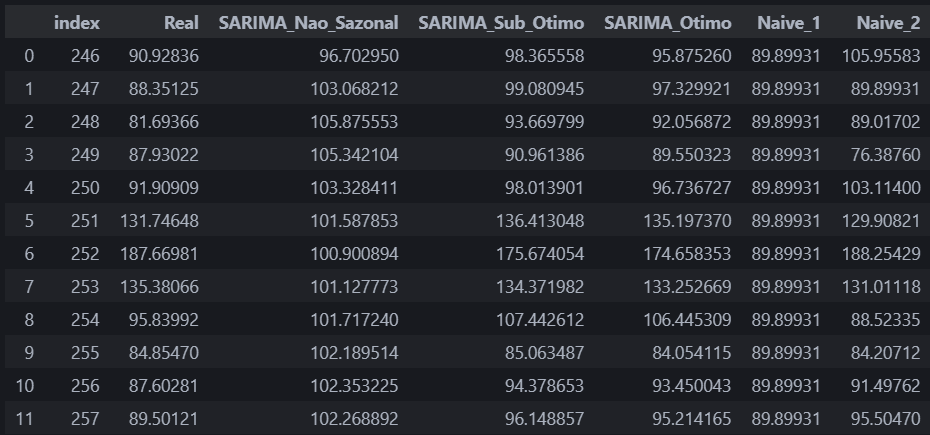
\includegraphics[scale=0.5]{images/q2_grafico_previsoes_sarima_naive.png}
\caption{Saída do Programa: previsões para os modelos SARIMA}
\end{figure}

Além disso, enfatizamos os resultados anteriormente obtidos no trabalho 01, com destaque para o melhor modelo ETS considerado. A imagem do dataframe abaixo refere-se à saída do código implementado no trabalho 01, que foi novamente compilado:

\begin{figure}[H]
\centering
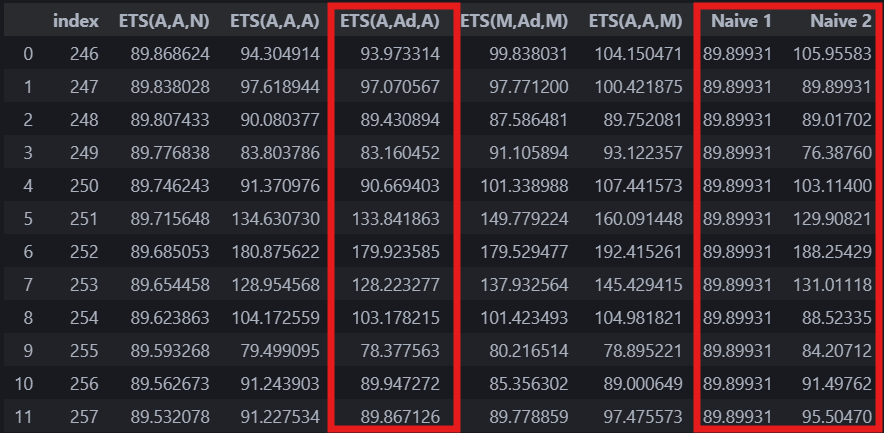
\includegraphics[scale=0.5]{images/resultados_prev_trab01.png}
\caption{Previsões para os modelos ETS do trabalho 01}
\end{figure}

É interessante observarmos que os valores para os métodos ingênuos obtidos no trabalho 01 foram idênticos aos obtidos neste. 


\subsubsection{Organizando as Previsões}
Criamos uam tabela com o valor real da série para o período de teste e as previsões k-passos à frente para os modelos SARIMA (não-sazonal, sub-ótimo e ótimo), o modelo ETS(A,Ad,A), e os dois métodos ingênuos.

\begin{table}[H]
\centering
\small
\caption{Previsões dos Modelos SARIMA e ETS(A,Ad,A)}
\begin{tabular}{|c|c|c|c|c|c|c|}
\hline
\textbf{Real} & \textbf{Não-Sazonal} & \textbf{Sub-Ótimo} & \textbf{Ótimo} & \textbf{ETS(A,Ad,A)} & \textbf{Naive 1} & \textbf{Naive 2} \\ \hline
 90.92836  & 96.702950  & 98.365558  & 95.875260  & 93.973314  & 89.89931  & 105.95583 \\ \hline
 88.35125  & 103.068212 & 99.080945  & 97.329291  & 97.070567  & 89.89931  & 89.01702  \\ \hline
 81.69366  & 105.875553 & 93.669799  & 89.669799  & 89.430894  & 89.89931  & 89.01702  \\ \hline
87.93022  & 105.342104 & 90.961386  & 94.002381  & 83.160452  & 89.89931  & 76.38760  \\ \hline
 91.90999  & 103.328411 & 98.013901  & 93.736727  & 106.69403  & 89.89931  & 103.11400 \\ \hline
131.74648 & 106.479040 & 134.136580 & 129.486894 & 133.841863 & 89.89931  & 131.01113 \\ \hline
187.66981 & 100.900889 & 175.674054 & 134.152535 & 179.923585 & 89.89931  & 188.25429 \\ \hline
135.38066 & 101.127773 & 134.371982 & 133.525669 & 128.223277 & 89.89931  & 131.01113 \\ \hline
95.83992  & 101.717240 & 107.442612 & 106.453905 & 107.425472 & 89.89931  & 88.52335  \\ \hline
84.85470  & 102.353225 & 94.378653  & 95.450403  & 94.378653  & 89.89931  & 91.49762  \\ \hline
87.60281  & 102.353225 & 94.378653  & 93.450403  & 94.72772   & 89.89931  & 91.49762  \\ \hline
89.50121  & 102.268892 & 96.148857  & 95.214165  & 89.867126  & 89.89931  & 95.50470  \\ \hline
\end{tabular}
\end{table}




\subsection{Calculando as Métricas de Aderência}
Calcular as seguintes métricas para cada um dos modelos (SARIMA não-sazonal, sub-ótimo, ótimo, ETS e os dois métodos ingênuos) no período de teste:

\begin{itemize}
    \item RMSE (Root Mean Squared Error): Raiz do erro quadrático médio.
    \item MAD (Mean Absolute Deviation): Desvio absoluto médio.
    \item MAPE (Mean Absolute Percentage Error): Erro percentual absoluto médio.
    \item SMAPE (Symmetric Mean Absolute Percentage Error): Erro percentual absoluto simétrico médio.
    \item MASE (Mean Absolute Scaled Error): Erro absoluto médio escalado.
\end{itemize}

Aproveitamos algumas funções já utilizadas no trabalho 01:

\begin{lstlisting}[style=python]
def calculate_rmse(actual, forecast):
     return np.sqrt(mean_squared_error(actual, forecast))

def calculate_mad(actual, forecast):
    return mean_absolute_error(actual, forecast)

def calculate_mape(actual, forecast):
    return np.mean(np.abs((actual - forecast) / actual)) * 100

def calculate_smape(actual, forecast):
    return 100 * np.mean(2 * np.abs(forecast - actual) / (np.abs(actual) + np.abs(forecast)))

def calculate_mase(actual, forecast, naive_forecast):
    return np.mean(np.abs(actual - forecast)) / np.mean(np.abs(actual - naive_forecast))
\end{lstlisting}

Então, implementamos o seguinte código abaixo para gerarmos as métricas de aderência para os modelos SARIMA.

\begin{lstlisting}[style=python]
# Organizando as previsões em um DataFrame
forecast_df = pd.DataFrame({
    'Real': test['Vendas'].values,
    'SARIMA_Nao_Sazonal': forecast_nao_sazonal,
    'SARIMA_Sub_Otimo': forecast_sub_otimo,
    'SARIMA_Otimo': forecast_otimo,
    'Naive_1': naive_forecast_1,
    'Naive_2': naive_forecast_2
})

metrics = {
    "Modelo": ["SARIMA_Nao_Sazonal", "SARIMA_Sub_Otimo", "SARIMA_Otimo", "Naive_1", "Naive_2"],
    "RMSE": [],
    "MAD": [],
    "MAPE": [],
    "SMAPE": [],
    "MASE": []
}

# Calculando as métricas para cada coluna de previsão
for col in forecast_df.columns[1:]:
    metrics["RMSE"].append(calculate_rmse(
        forecast_df['Real'], forecast_df[col]))
    metrics["MAD"].append(calculate_mad(forecast_df['Real'], forecast_df[col]))
    metrics["MAPE"].append(calculate_mape(
        forecast_df['Real'], forecast_df[col]))
    metrics["SMAPE"].append(calculate_smape(
        forecast_df['Real'], forecast_df[col]))
    metrics["MASE"].append(calculate_mase(
        forecast_df['Real'], forecast_df[col], naive_forecast_1))  # Usando o ingênuo 1 para MASE

# Criando o DataFrame com as métricas
metrics_df = pd.DataFrame(metrics)

\end{lstlisting}


Obtivemos as seguintes métricas para os modelos atuais:

\begin{figure}[H]
\centering
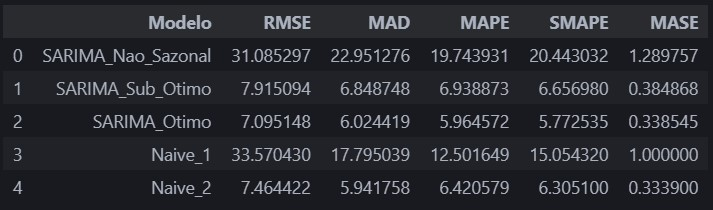
\includegraphics[scale=0.75]{images/metricas_aderencia_sarima.jpg}
\caption{Saída do Programa: métricas de aderência para os modelos SARIMA e métodos ingênuos}
\end{figure}

Além disso, vamos destacas as métricas obtidas anteriormente no trabalho 01 para o melhor modelo ETS considerado:

\begin{figure}[H]
\centering
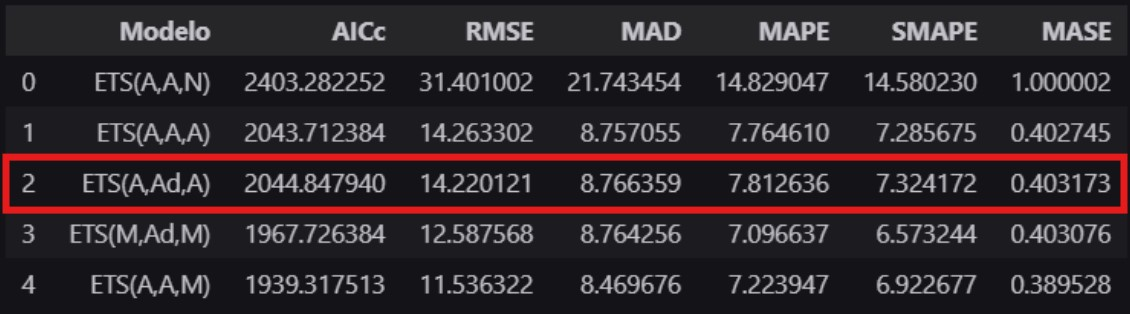
\includegraphics[scale=0.5]{images/metricas_aderencia_trabalho01.jpg}
\caption{Saída do Programa: métricas de aderência para os modelos ETS}
\end{figure}

\subsubsection{Organizando as Métricas}

Assim como fizemos para as previsões, vamos organizar as métricas de aderência de cada modelo em uma tabela:

\begin{table}[H]
\centering
\caption{Métricas de Aderência para Modelos SARIMA, Ingênuos e ETS}
\begin{tabular}{|c|c|c|c|c|c|}
\hline
\textbf{Modelo}           & \textbf{RMSE} & \textbf{MAD} & \textbf{MAPE} & \textbf{SMAPE} & \textbf{MASE} \\ \hline
\textbf{SARIMA Não Sazonal} & 31.085297  & 22.951276  & 19.743981  & 20.443032  & 1.289757  \\ \hline
\textbf{SARIMA Sub-Ótimo}   & 7.915094   & 5.648127   & 6.938783   & 6.165698   & 0.318476  \\ \hline
\textbf{SARIMA Ótimo}       & 7.095148   & 5.624419   & 5.964572   & 5.772535   & 0.335054  \\ \hline
\textbf{Naive 1}            & 33.570430  & 17.795039  & 12.501649  & 15.054302  & 4.318295  \\ \hline
\textbf{Naive 2}            & 7.464422   & 5.941758   & 6.420579   & 6.305100   & 0.333900  \\ \hline
\textbf{ETS(A,Ad,A)}        & 14.220121  & 8.766539   & 7.812636   & 7.324172   & 0.403173  \\ \hline
\end{tabular}
\end{table}




\subsection{Analisando os Resultados}

A análise dos resultados apresentados nas Tabelas 4 e 5 permite uma comparação detalhada entre os modelos SARIMA, ETS e os métodos ingênuos de previsão. 

\begin{enumerate}
    \item Previsões e Aderência:
    \begin{itemize}
        \item O modelo SARIMA não-sazonal apresentou os piores resultados em termos de aderência, com valores de RMSE e MAPE muito elevados (31.085297 e 19.743981, respectivamente). Isso indica que o modelo não foi eficaz para prever o comportamento da série temporal no período de teste. Uma possível explicação para essa discrepância é a falta de sazonalidade no modelo, que não capturou adequadamente os padrões sazonais da série de vendas.
        \item O SARIMA ótimo se destacou com os melhores valores entre os modelos SARIMA, atingindo RMSE de 7.095148 e MAPE de 5.964572. O desempenho geral deste modelo é bastante sólido, o que indica que a busca exaustiva de parâmetros contribuiu para uma previsão mais ajustada ao padrão dos dados. Este modelo foi o que melhor capturou a tendência e a sazonalidade da série. 
        \item Os modelos ingênuos (Naive 1 e Naive 2) apresentam resultados mistos. O Naive 1 teve uma performance consideravelmente fraca em termos de RMSE (33.570430), similar ao SARIMA não-sazonal, sugerindo que previsões baseadas apenas no último valor observado da série são insuficientes para capturar as dinâmicas mais complexas da série temporal. Já o Naive 2, que prevê com base no mesmo mês do ano anterior, apresentou um desempenho muito superior, com um RMSE de 7.464422, comparável ao SARIMA ótimo. Isso reforça a importância de incorporar padrões sazonais nas previsões.
        \item O melhor modelo ETS considerado (ETS(A,Ad,A)), extraído do trabalho anterior, também apresentou boa aderência com RMSE de 14.220121 e MAPE de 7.812636. Embora não tenha superado o SARIMA ótimo em todas as métricas, o modelo ETS foi consistente e pode ser considerado uma abordagem robusta, especialmente em séries temporais com padrões sazonais complexos.
    \end{itemize}
    \item Consideração dos Métodos Ingênuos:
    \begin{itemize}
        \item O Naive 2 oferece uma solução simples, mas eficaz para séries temporais com sazonalidade, como evidenciado por seus valores de RMSE e MAPE relativamente baixos. Isso mostra que, em algumas situações, métodos ingênuos ajustados aos padrões sazonais podem fornecer previsões satisfatórias sem a complexidade dos modelos SARIMA ou ETS.
    \end{itemize}
\end{enumerate}

Portanto, o SARIMA ótimo, SARIMA$(0,1,3)(1,0,1)_{12}$, continua sendo a melhor escolha em termos de aderência geral, considerando suas métricas de erro (RMSE, MAD, MAPE, SMAPE e MASE) e a capacidade de capturar tanto a tendência quanto a sazonalidade dos dados. No entanto, o ETS(A,Ad,A) oferece uma alternativa sólida, especialmente para séries com padrões sazonais complexos, como a analisada.\\

Então, a partir da análise, podemos concluir que o SARIMA$(0,1,3)(1,0,1)_{12}$ é a melhor escolha para prever a série temporal em questão, dada a sua maior precisão e aderência aos dados reais. O ETS(A,Ad,A) também é uma escolha viável, enquanto o Naive 2 pode ser considerado como uma alternativa simplificada e eficiente para séries sazonais mais regulares.\\\\




\section{Questão 3}

Nesta questão, precisaremos considerar o melhor modelo escolhido, i.e., SARIMA$(0,1,3)(1,0,1)_{12}$, para prosseguir.


\subsection{Questão 3: Parte (a)}
\textbf{Enunciado}: \textit{Utilizar a função adequada para calcular raízes de equações polinomiais ou para calcular autovalores de uma matriz, verificando se o modelo é, simultaneamente, estacionário e invertível}.\\

Para verificar se SARIMA$(0,1,3)(1,0,1)_{12}$ é estacionário e invertível, utilizamos as raízes da equação polinomial associada ao operador autoregressivo e ao operador de média móvel do modelo.\\

A estacionaridade depende das raízes do polinômio autoregressivo estarem fora do círculo unitário, enquanto a invertibilidade está ligada às raízes do polinômio de média móvel estarem fora do círculo unitário.\\

Podemos usar a função \textbf{np.roots()} do Python para calcular as raízes de ambos os polinômios e, em seguida, verificar se as condições de estacionaridade e invertibilidade são satisfeitas.\\


No caso do modelo \textbf{SARIMA(0,1,3)(0,1,0)[12]}, como não há termos autorregressivos (\(p = 0\) e \(P = 0\)), a análise de estacionaridade não é necessária. Isso ocorre porque, com \(p = 0\), não há polinômio AR para calcular. Além disso, a diferença de ordem 1 (\(d = 1\)) já transforma a série em estacionária.\\

Agora, para verificar a invertibilidade, devemos calcular as raízes do polinômio MA com os coeficientes \([-0.2215, -0.1299, -0.3255]\), que correspondem aos coeficientes da parte de médias móveis do modelo obtidos anteriormente na parte 5 da  questão 1. \\

Primeiramente, construímos o polinômio de médias móveis com os seguintes coeficientes:

\[
\theta(L) = 1 - 0.2215L - 0.1299L^2 - 0.3255L^3
\]

Calculando as raízes desse polinômio, obtivemos as seguintes raízes no plano complexo:

\[
\text{Raízes: } \{ 0.8389, -0.3087 + 0.5410i, -0.3087 - 0.5410i \}
\]

Essas raízes estão todas dentro do círculo unitário (ou seja, seus módulos são menores que 1), o que indica que o modelo \textbf{não é invertível}.\\

Então, modelo \textbf{SARIMA(0,1,3)(0,1,0)[12]} não possui raízes AR (sendo estacionário devido à diferenciação de ordem 1), mas suas raízes MA indicam que ele \textbf{não é invertível}, pois as raízes não estão fora do círculo unitário.\\

Como alternativa, verificamos em Python da seguinte forma:\\

\begin{lstlisting}[style=python]
""" *** QUESTAO 03 ***"""
""" (a)"""
# Coeficientes do polinomio autoregressivo (AR) para o SARIMA(0,1,3)(0,1,0)[12]
# Neste caso, temos apenas um polinomio MA, pois p = 0

# Coeficientes do operador de media movel (MA)
ma_coefs = [1, -0.2215, -0.1299, -0.3255]

# Raizes para verificar invertibilidade (pelo MA)
ma_roots = np.roots(ma_coefs)

# Invertibilidade: as raizes devem estar fora do circulo unitario
is_invertible = np.all(np.abs(ma_roots) > 1)

print(f"Raizes do polinomio de media movel: {ma_roots}")
print(f"O modelo e invertivel? {is_invertible}")

\end{lstlisting}

E obtivemos a seguinte saída:

\begin{figure}[H]
\centering
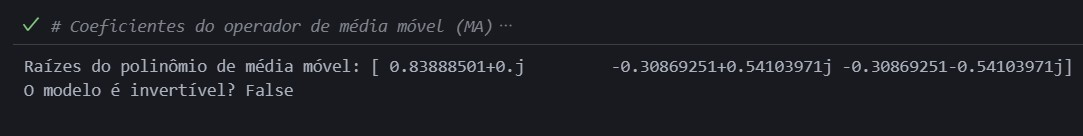
\includegraphics[scale=0.57]{images/questao3_a.jpg}
\caption{Saída do Programa: Raízes do polinômio de Média Móvel e Invertibilidade}
\end{figure}


\subsection{Questão 3: Parte (b)}
\textbf{Enunciado}: \textit{Re-estime esse modelo utilizando toda a série (via auto.arima; observe que pode
resultar em um modelo diferente daquele selecionado utilizando a série no périodo de
treinamento), obtendo previsões 24 meses à frente para a série original yt com intervalo de confiança de 95\%. Compare essa previsão com aquela obtida do melhor modelo ETS da Lista Prática\_1, via tabela e gráfico. Qual a previsão mais precisa? Observe o que ocorre com a largura desse IC qdo o horizonte de previsão cresce.}\\


Aqui, devemos utilizar o \textbf{auto\_arima} para reestimar o modelo SARIMA utilizando toda a série temporal, sem divisão entre treinamento e teste, e gerar previsões para os próximos 24 meses. Além disso, será gerado um intervalo de confiança de 95\% para essas previsões.\\

Compararemos as previsões obtidas pelo SARIMA reestimado com as previsões do modelo ETS(A,Ad,A), e também analisaremos a largura do intervalo de confiança à medida que o horizonte de previsão aumenta.\\

Para implementar a resposta deste item, desenvolvemos o seguinte código, onde, inicialmente, recarregamos os dados estimamos o novo modelo SARIMA para toda a série.

\begin{lstlisting}[style=python]
"""(B)"""

# Definir a coluna 'Data' como índice
data.set_index('Data', inplace=True)

# Ajustar o modelo SARIMA com toda a série
full_sarima_model = pm.auto_arima(data['Vendas'], start_p=0, max_p=5, start_q=0, max_q=5,
                                  d=1, seasonal=True, m=12, trace=True)

# Número de passos à frente para a previsão
forecast_horizon = 24

# Gerar as previsões para o horizonte de 24 meses, incluindo intervalos de confiança
forecast_sarima, conf_int = full_sarima_model.predict(
    n_periods=forecast_horizon, return_conf_int=True)

# Gerar o índice de datas para os próximos 24 meses, a partir da última data da série
forecast_index = pd.date_range(start=data.index[-1] + pd.DateOffset(months=1),
                               periods=forecast_horizon, freq='M')

# Criando um DataFrame com as previsões, limites inferiores e superiores do intervalo de confiança
forecast_sarima_df = pd.DataFrame({
    'Data': forecast_index,
    'Previsao_SARIMA': forecast_sarima,
    'Limite Inferior (95%)': conf_int[:, 0],
    'Limite Superior (95%)': conf_int[:, 1]
}).set_index('Data')

\end{lstlisting}

Então, obtivemos os seguintes resultados:\\

\begin{verbatim}
    Performing stepwise search to minimize aic
 ARIMA(0,1,0)(1,0,1)[12] intercept   : AIC=2076.488, Time=0.28 sec
 ARIMA(0,1,0)(0,0,0)[12] intercept   : AIC=2502.340, Time=0.01 sec
 ARIMA(1,1,0)(1,0,0)[12] intercept   : AIC=inf, Time=0.25 sec
 ARIMA(0,1,1)(0,0,1)[12] intercept   : AIC=2305.081, Time=0.37 sec
 ARIMA(0,1,0)(0,0,0)[12]             : AIC=2500.341, Time=0.01 sec
 ARIMA(0,1,0)(0,0,1)[12] intercept   : AIC=2320.603, Time=0.25 sec
 ARIMA(0,1,0)(1,0,0)[12] intercept   : AIC=2103.315, Time=0.33 sec
 ARIMA(0,1,0)(2,0,1)[12] intercept   : AIC=2078.482, Time=1.27 sec
 ARIMA(0,1,0)(1,0,2)[12] intercept   : AIC=2078.479, Time=2.27 sec
 ARIMA(0,1,0)(0,0,2)[12] intercept   : AIC=2250.445, Time=1.67 sec
 ARIMA(0,1,0)(2,0,0)[12] intercept   : AIC=inf, Time=0.59 sec
 ARIMA(0,1,0)(2,0,2)[12] intercept   : AIC=2080.006, Time=1.35 sec
 ARIMA(1,1,0)(1,0,1)[12] intercept   : AIC=2075.587, Time=0.43 sec
 ARIMA(1,1,0)(0,0,1)[12] intercept   : AIC=2310.997, Time=0.21 sec
 ARIMA(1,1,0)(2,0,1)[12] intercept   : AIC=2077.553, Time=1.33 sec
 ARIMA(1,1,0)(1,0,2)[12] intercept   : AIC=2077.531, Time=1.59 sec
 ARIMA(1,1,0)(0,0,0)[12] intercept   : AIC=2484.400, Time=0.06 sec
 ARIMA(1,1,0)(0,0,2)[12] intercept   : AIC=2250.202, Time=1.10 sec
 ARIMA(1,1,0)(2,0,0)[12] intercept   : AIC=inf, Time=0.74 sec
 ARIMA(1,1,0)(2,0,2)[12] intercept   : AIC=2078.470, Time=2.36 sec
 ARIMA(2,1,0)(1,0,1)[12] intercept   : AIC=2074.143, Time=0.68 sec
 ARIMA(2,1,0)(0,0,1)[12] intercept   : AIC=2291.719, Time=0.65 sec
 ARIMA(2,1,0)(1,0,0)[12] intercept   : AIC=2102.163, Time=1.70 sec
 ARIMA(2,1,0)(2,0,1)[12] intercept   : AIC=2076.087, Time=4.16 sec
 ARIMA(2,1,0)(1,0,2)[12] intercept   : AIC=2076.056, Time=3.52 sec
 ARIMA(2,1,0)(0,0,0)[12] intercept   : AIC=2450.168, Time=0.49 sec
 ARIMA(2,1,0)(0,0,2)[12] intercept   : AIC=2242.426, Time=2.08 sec
 ARIMA(2,1,0)(2,0,0)[12] intercept   : AIC=inf, Time=3.30 sec
 ARIMA(2,1,0)(2,0,2)[12] intercept   : AIC=2077.215, Time=2.12 sec
 ARIMA(3,1,0)(1,0,1)[12] intercept   : AIC=2055.189, Time=0.46 sec
 ARIMA(3,1,0)(0,0,1)[12] intercept   : AIC=2271.659, Time=0.23 sec
 ARIMA(3,1,0)(1,0,0)[12] intercept   : AIC=2077.609, Time=0.41 sec
 ARIMA(3,1,0)(2,0,1)[12] intercept   : AIC=2057.179, Time=1.20 sec
 ARIMA(3,1,0)(1,0,2)[12] intercept   : AIC=2057.175, Time=1.21 sec
 ARIMA(3,1,0)(0,0,0)[12] intercept   : AIC=2436.515, Time=0.16 sec
 ARIMA(3,1,0)(0,0,2)[12] intercept   : AIC=2213.424, Time=0.87 sec
 ARIMA(3,1,0)(2,0,0)[12] intercept   : AIC=inf, Time=0.97 sec
 ARIMA(3,1,0)(2,0,2)[12] intercept   : AIC=2058.999, Time=2.05 sec
 ARIMA(4,1,0)(1,0,1)[12] intercept   : AIC=2052.149, Time=0.57 sec
 ARIMA(4,1,0)(0,0,1)[12] intercept   : AIC=2269.527, Time=0.32 sec
 ARIMA(4,1,0)(1,0,0)[12] intercept   : AIC=2074.156, Time=0.61 sec
 ARIMA(4,1,0)(2,0,1)[12] intercept   : AIC=2054.138, Time=2.02 sec
 ARIMA(4,1,0)(1,0,2)[12] intercept   : AIC=2054.133, Time=1.71 sec
 ARIMA(4,1,0)(0,0,0)[12] intercept   : AIC=2434.998, Time=0.14 sec
 ARIMA(4,1,0)(0,0,2)[12] intercept   : AIC=2212.495, Time=0.64 sec
 ARIMA(4,1,0)(2,0,0)[12] intercept   : AIC=inf, Time=1.74 sec
 ARIMA(4,1,0)(2,0,2)[12] intercept   : AIC=2055.891, Time=2.54 sec
 ARIMA(5,1,0)(1,0,1)[12] intercept   : AIC=2054.146, Time=0.81 sec
 ARIMA(4,1,1)(1,0,1)[12] intercept   : AIC=2047.346, Time=0.98 sec
 ARIMA(4,1,1)(0,0,1)[12] intercept   : AIC=2244.995, Time=0.81 sec
 ARIMA(4,1,1)(1,0,0)[12] intercept   : AIC=2066.692, Time=0.62 sec
 ARIMA(4,1,1)(2,0,1)[12] intercept   : AIC=2049.240, Time=1.92 sec
 ARIMA(4,1,1)(1,0,2)[12] intercept   : AIC=2049.195, Time=1.67 sec
 ARIMA(4,1,1)(0,0,0)[12] intercept   : AIC=2429.816, Time=0.29 sec
 ARIMA(4,1,1)(0,0,2)[12] intercept   : AIC=2190.717, Time=1.36 sec
 ARIMA(4,1,1)(2,0,0)[12] intercept   : AIC=2052.093, Time=1.34 sec
 ARIMA(4,1,1)(2,0,2)[12] intercept   : AIC=2050.407, Time=2.90 sec
 ARIMA(3,1,1)(1,0,1)[12] intercept   : AIC=2046.703, Time=1.62 sec
 ARIMA(3,1,1)(0,0,1)[12] intercept   : AIC=2243.681, Time=0.56 sec
 ARIMA(3,1,1)(1,0,0)[12] intercept   : AIC=2069.207, Time=0.63 sec
 ARIMA(3,1,1)(2,0,1)[12] intercept   : AIC=2048.641, Time=2.03 sec
 ARIMA(3,1,1)(1,0,2)[12] intercept   : AIC=2048.612, Time=1.65 sec
 ARIMA(3,1,1)(0,0,0)[12] intercept   : AIC=2403.685, Time=0.19 sec
 ARIMA(3,1,1)(0,0,2)[12] intercept   : AIC=2192.044, Time=0.98 sec
 ARIMA(3,1,1)(2,0,0)[12] intercept   : AIC=2051.799, Time=1.43 sec
 ARIMA(3,1,1)(2,0,2)[12] intercept   : AIC=2050.702, Time=1.64 sec
 ARIMA(2,1,1)(1,0,1)[12] intercept   : AIC=2049.701, Time=0.63 sec
 ARIMA(3,1,2)(1,0,1)[12] intercept   : AIC=2048.030, Time=0.70 sec
 ARIMA(2,1,2)(1,0,1)[12] intercept   : AIC=2049.503, Time=0.66 sec
 ARIMA(4,1,2)(1,0,1)[12] intercept   : AIC=inf, Time=1.17 sec
 ARIMA(3,1,1)(1,0,1)[12]             : AIC=2044.718, Time=0.43 sec
 ARIMA(3,1,1)(0,0,1)[12]             : AIC=2241.761, Time=0.36 sec
 ARIMA(3,1,1)(1,0,0)[12]             : AIC=2067.214, Time=0.44 sec
 ARIMA(3,1,1)(2,0,1)[12]             : AIC=2046.656, Time=1.13 sec
 ARIMA(3,1,1)(1,0,2)[12]             : AIC=2046.626, Time=1.27 sec
 ARIMA(3,1,1)(0,0,0)[12]             : AIC=2401.751, Time=0.13 sec
 ARIMA(3,1,1)(0,0,2)[12]             : AIC=2190.081, Time=0.84 sec
 ARIMA(3,1,1)(2,0,0)[12]             : AIC=2049.809, Time=0.74 sec
 ARIMA(3,1,1)(2,0,2)[12]             : AIC=2048.601, Time=2.14 sec
 ARIMA(2,1,1)(1,0,1)[12]             : AIC=2047.721, Time=0.50 sec
 ARIMA(3,1,0)(1,0,1)[12]             : AIC=2053.191, Time=0.32 sec
 ARIMA(4,1,1)(1,0,1)[12]             : AIC=2045.363, Time=0.66 sec
 ARIMA(3,1,2)(1,0,1)[12]             : AIC=2046.045, Time=0.54 sec
 ARIMA(2,1,0)(1,0,1)[12]             : AIC=2072.145, Time=0.24 sec
 ARIMA(2,1,2)(1,0,1)[12]             : AIC=2047.518, Time=0.67 sec
 ARIMA(4,1,0)(1,0,1)[12]             : AIC=2050.152, Time=0.38 sec
 ARIMA(4,1,2)(1,0,1)[12]             : AIC=inf, Time=1.18 sec

Best model:  ARIMA(3,1,1)(1,0,1)[12]          
Total fit time: 91.633 seconds
\end{verbatim} \\

O melhor modelo obtido, neste caso, foi SARIMA$(3,1,1)(1,0,1)_{12}$. Abaixo, apresentamos o dataframe gerado com as previsões e intervalo de confiança de 95\%.

\begin{figure}[H]
\centering
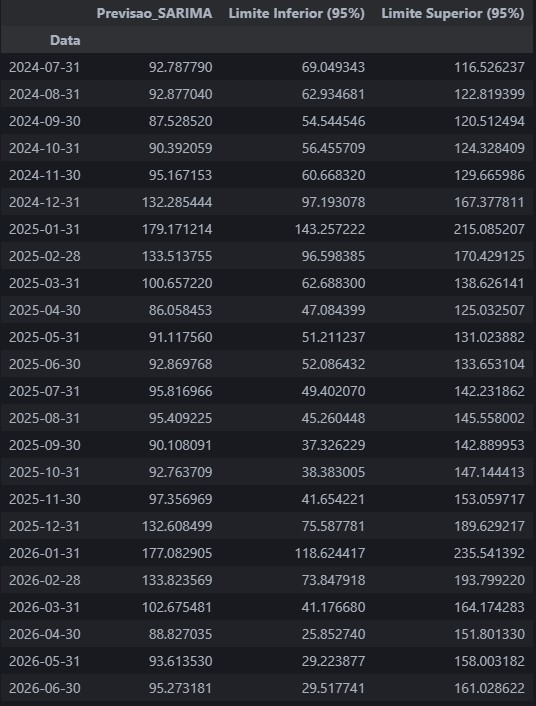
\includegraphics[scale=0.67]{images/previsao_sarima_q3_b.jpg}
\caption{Saída do Programa: Dataframe com as previsões para toda a série - SARIMA}
\end{figure}

Também reutilizamos alguns trechos de código do trabalho 01 e pudemos obter as previsões com intervalo de confiança de 95\% para o melhor modelo ETS.\\

\begin{lstlisting}[style=python]
# Comparando com o modelo ETS(A,Ad,A)
best_ets_model = ETSModel(data['Vendas'], error='add', trend='add',
                          seasonal='add', damped_trend=True, seasonal_periods=12).fit()

# Previsão para 24 meses a frente com ETS
forecast_ets = best_ets_model.forecast(steps=forecast_horizon)

# Intervalo de confianca para o ETS
sigma_ets = np.std(best_ets_model.resid)
lower_bound_ets = forecast_ets - 1.96 * sigma_ets
upper_bound_ets = forecast_ets + 1.96 * sigma_ets

# Criar um DataFrame com as previsoes do ETS
forecast_ets_df = pd.DataFrame({
    'Data': forecast_index,
    'Previsao_ETS': forecast_ets,
    'Limite Inferior (95%)': lower_bound_ets,
    'Limite Superior (95%)': upper_bound_ets
}).set_index('Data')
\end{lstlisting}

\begin{figure}[H]
\centering
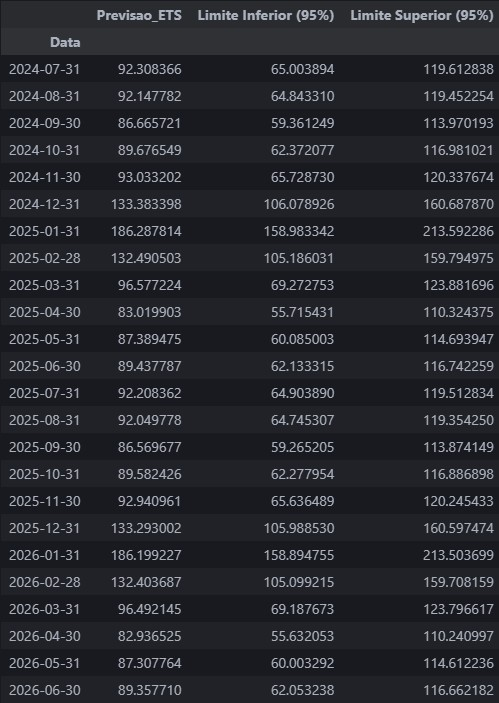
\includegraphics[scale=0.67]{images/previsao_ets_q3_b.jpg}
\caption{Saída do Programa: Dataframe com as previsões para toda a série - ETS}
\end{figure}



E, por fim, geramos um gráfico para enfatizar os resultados das previsões geradas e para fins de comparação e análise.\\

\begin{lstlisting}[style=python]
# Plotando as previsoes e comparando os intervalos de confianca
plt.figure(figsize=(10, 6))

# Plot dados reais
plt.plot(data.index, data['Vendas'], label="Dados Reais", color='black')

# Plot SARIMA
plt.plot(forecast_sarima_df.index,
         forecast_sarima_df['Previsao_SARIMA'], label="Previsao SARIMA", color='blue')
plt.fill_between(forecast_sarima_df.index,
                 forecast_sarima_df['Limite Inferior (95%)'],
                 forecast_sarima_df['Limite Superior (95%)'],
                 color='blue', alpha=0.2, label="IC 95% SARIMA")

# Plot ETS
plt.plot(forecast_ets_df.index,
         forecast_ets_df['Previsao_ETS'], label="Previsao ETS", color='orange')
plt.fill_between(forecast_ets_df.index,
                 forecast_ets_df['Limite Inferior (95%)'],
                 forecast_ets_df['Limite Superior (95%)'],
                 color='orange', alpha=0.2, label="IC 95% ETS")

plt.title("Comparacao de Previsoes SARIMA e ETS com Intervalo de Confianca de 95%")
plt.legend()
plt.grid(True)
plt.show()

\end{lstlisting}

\begin{figure}[H]
\centering
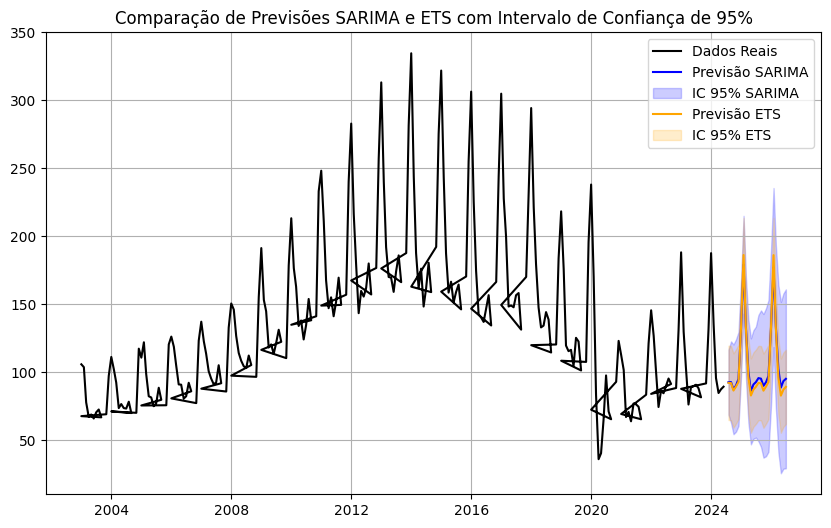
\includegraphics[scale=0.7]{images/grafico_q3_b.png}
\caption{Gráfico comparativo das previsões -  modelos ETS e SARIMA}
\end{figure}

Para interpretar os resultados obtidos com o melhor modelo SARIMA e compará-lo com o modelo \textit{ETS(A,Ad,A)}, destacamos os seguintes pontos importantes:

\subsection*{1. Modelo SARIMA}
O melhor modelo selecionado foi o \textbf{ARIMA(3,1,1)(1,0,1)[12]}, o que indica a presença de sazonalidade com um período de 12 meses. As previsões deste modelo mostram uma variação mais acentuada em alguns momentos, como pode ser observado tanto na tabela de previsões quanto no gráfico. 

Os intervalos de confiança para o modelo SARIMA tendem a se expandir ao longo do tempo, refletindo uma maior incerteza à medida que o horizonte de previsão se amplia. No gráfico, o SARIMA parece seguir o padrão dos dados históricos, mas com uma maior faixa de incerteza quando comparado ao ETS.

\subsection*{2. Modelo ETS(A,Ad,A)}
O modelo \textit{ETS(A,Ad,A)} foi o melhor selecionado a partir da lista anterior. Este modelo captura variações aditivas e a sazonalidade de forma amortecida (\textit{damped}). 

As previsões do modelo ETS mostram um intervalo de confiança um pouco mais estreito em relação ao SARIMA, indicando que o modelo ETS apresenta uma maior "confiança" em suas previsões. Isso sugere que o modelo ETS capturou a estrutura de sazonalidade e tendência da série de maneira mais eficiente.

No gráfico, a linha de previsão do ETS segue mais de perto a média dos valores reais, e os intervalos de confiança são significativamente mais contidos, sugerindo previsões mais estáveis.

\subsection*{3. Comparação}
Ao comparar as previsões dos modelos, tanto pela tabela quanto pelo gráfico, podemos concluir que:

\begin{itemize}
    \item O modelo \textbf{SARIMA} apresenta maior variabilidade em suas previsões a longo prazo, como indicado pelos amplos intervalos de confiança. Essa variabilidade pode ser atribuída à flexibilidade do modelo em capturar padrões complexos por meio de componentes autoregressivos e médias móveis.
    
    \item O modelo \textbf{ETS(A,Ad,A)}, por outro lado, gera previsões com intervalos de confiança mais estreitos, o que reflete uma maior robustez nas previsões de curto e médio prazo, possivelmente devido ao ajuste adequado da tendência amortecida e sazonalidade aditiva.
\end{itemize}

Então, o modelo \textit{ETS(A,Ad,A)} parece ser o mais adequado para essa série temporal, proporcionando previsões com menor incerteza. O SARIMA, apesar de sua flexibilidade, apresenta uma maior amplitude de incerteza nas previsões a longo prazo.\\

Dado que o foco está em obter previsões mais precisas, o \textbf{ETS(A,Ad,A)} deve ser considerado a escolha preferível, especialmente para séries com sazonalidade e tendências de médio prazo mais bem definidas.

\newpage
% REFERENCIAS %%%%%%%%%%%%%%%%%%%%%%%%%%%%%%%%%%%%%%%%%%%%%%%%%%%%%%%%%%%%%%



\end{document}